% \section{Representation}

% \begin{exercise}[1.1.9]
% Let $K$ be a field. Show that the ring $M_n(K)$ has no two-sided ideals other than $\{0\}$ and $M_n(K)$.
% \end{exercise}

% \begin{proof}
% Let $I\lhd M_n(K)$ be a two-sided ideal. If $I=\{0\}$ we are done, so assume $I\ne\{0\}$ and pick a nonzero $A=(a_{ij})\in I$.
% Choose indices $p,q$ with $a_{pq}\neq 0$. For $1\le i,j\le n$, let $E_{ij}$ denote the standard matrix unit (a $1$ at $(i,j)$ and $0$ elsewhere).

% Because $I$ is two-sided, for any $i,j$ we have
% \[
% E_{ip}\,A\,E_{qj}\ \in\ I.
% \]
% But a direct multiplication shows
% \[
% E_{ip}\,A\,E_{qj}\ =\ a_{pq}\,E_{ij}.
% \]
% Since $a_{pq}\in K^\times$, it follows that $E_{ij} = a_{pq}^{-1}\,E_{ip}AE_{qj}\in I$ for all $i,j$.
% Thus every matrix unit $E_{ij}$ lies in $I$, and hence any matrix
% \(
% X=\sum_{i,j} x_{ij}E_{ij}
% \)
% also lies in $I$. Therefore $I=M_n(K)$.

% We conclude that the only two-sided ideals are $\{0\}$ and $M_n(K)$; i.e.\ $M_n(K)$ is a simple ring.
% \end{proof}


% \begin{definition}[$K$-algebra]
% A \emph{$K$-algebra} is a ring $R$ whose underlying additive group is a $K$-vector space and whose multiplication
% \[
% \mu: R\times R \to R
% \]
% is $K$-bilinear:
% \[
% a(xy)=(ax)y = x(ay), \qquad \forall a\in K,\, x,y\in R.
% \]
% We consider only unital $K$-algebras, that is, algebras with multiplicative identity $1_R$.
% \end{definition}

% \begin{definition}[Ideals in a $K$-algebra]
% Let $R$ be a $K$-algebra.
% \begin{itemize}
%     \item A \emph{left ideal} of $R$ is a $K$-linear subspace $I\subseteq R$ such that
%     \[
%     RI \subseteq I.
%     \]
%     \item A \emph{right ideal} of $R$ is a $K$-linear subspace $I\subseteq R$ satisfying
%     \[
%     IR \subseteq I.
%     \]
%     \item A \emph{two-sided ideal} is a subspace $I$ which is both a left and a right ideal.
% \end{itemize}
% \end{definition}

% \begin{remark}
% In a commutative $K$-algebra, the notions of left, right, and two-sided ideals coincide.  
% However, in noncommutative algebras such as $M_n(K)$, they differ.
% \end{remark}

% \section{Examples in Matrix Algebras}

% Let $R = M_n(K)$.

% \subsection*{Example 1: Left but not right ideal}
% \[
% I_L = 
% \left\{
% \begin{pmatrix}
% a & 0 \\[2pt]
% b & 0
% \end{pmatrix}
% : a,b\in K
% \right\}.
% \]
% Then:
% \begin{itemize}
%     \item $I_L$ is a linear subspace.
%     \item For all $A\in R$ and $X\in I_L$, $AX$ still has second column zero, hence $AX\in I_L$.
%     \item For $X\in I_L$ and $A\in R$, $XA$ may have nonzero second column, so $XA\notin I_L$ in general.
% \end{itemize}
% Thus $I_L$ is a \emph{left ideal}, but not a right ideal.

% \subsection*{Example 2: Right but not left ideal}
% \[
% I_R = 
% \left\{
% \begin{pmatrix}
% a & b \\[2pt]
% 0 & 0
% \end{pmatrix}
% : a,b\in K
% \right\}.
% \]
% Then:
% \begin{itemize}
%     \item $I_R$ is a linear subspace.
%     \item For all $X\in I_R$ and $A\in R$, $XA$ has second row zero, hence $XA\in I_R$.
%     \item But $AX$ may have nonzero second row, so $AX\notin I_R$.
% \end{itemize}
% Hence $I_R$ is a \emph{right ideal}, but not a left ideal.

% \subsection*{Example 3: General Form in $M_n(K)$}
% \begin{align*}
% I_j &= \{A\in M_n(K)\mid \text{columns } j+1,\dots,n\text{ are zero}\}, \\
% J_i &= \{A\in M_n(K)\mid \text{rows } i+1,\dots,n\text{ are zero}\}.
% \end{align*}
% Then $I_j$ is left (not right), while $J_i$ is right (not left).

% \section{Examples in $\mathrm{End}_K(V)$}

% Let $V$ be a finite-dimensional $K$-vector space and $R=\mathrm{End}_K(V)$.

% \subsection*{Example 4: Maps with image in a fixed subspace}
% Let $W\subsetneq V$ and define
% \[
% I_R = \{f\in R\mid \mathrm{Im}(f)\subseteq W\}.
% \]
% Then:
% \begin{itemize}
%     \item $I_R$ is a right ideal: $(f h)(V)\subseteq \mathrm{Im}(f)\subseteq W$ for all $h\in R$.
%     \item It is not a left ideal: for $h\in R$, $(h f)(V)=h(\mathrm{Im}(f))$ may not lie in $W$.
% \end{itemize}

% \subsection*{Example 5: Maps killing a fixed subspace}
% \[
% I_L = \{f\in R\mid W\subseteq \ker(f)\}.
% \]
% Then:
% \begin{itemize}
%     \item $I_L$ is a left ideal: $(h f)(w)=h(f(w))=0$ for all $w\in W$, $h\in R$.
%     \item It is not a right ideal: $(f h)(w)=f(h(w))$ may fail to vanish on $W$.
% \end{itemize}

% \subsection*{Concrete Matrix Forms (for $V=K^2$, $W=\mathrm{span}\{e_1\}$)}
% \[
% I_L =
% \left\{
% \begin{pmatrix}
% 0 & a \\[2pt]
% 0 & b
% \end{pmatrix}
% : a,b\in K
% \right\}, \qquad
% I_R =
% \left\{
% \begin{pmatrix}
% a & b \\[2pt]
% 0 & 0
% \end{pmatrix}
% : a,b\in K
% \right\}.
% \]
% Then $I_L$ is left (not right), $I_R$ is right (not left).

% \section{Examples in the Upper-Triangular Algebra}

% Let
% \[
% R=
% \left\{
% \begin{pmatrix}
% a & b\\[2pt]
% 0 & c
% \end{pmatrix}
% : a,b,c\in K
% \right\}.
% \]
% Define
% \[
% J=
% \left\{
% \begin{pmatrix}
% a & 0\\[2pt]
% 0 & 0
% \end{pmatrix}
% : a\in K
% \right\}, \qquad
% K=
% \left\{
% \begin{pmatrix}
% 0 & 0\\[2pt]
% 0 & c
% \end{pmatrix}
% : c\in K
% \right\}.
% \]
% Then:
% \begin{itemize}
%     \item $J$ is a left ideal (not right),
%     \item $K$ is a right ideal (not left).
% \end{itemize}

% \section{Example in a Path Algebra}

% Let $Q: 1 \xrightarrow{\alpha} 2$ be a quiver and $KQ$ its path algebra, with basis $\{e_1,e_2,\alpha\}$.
% Multiplication satisfies
% \[
% e_1\alpha=\alpha,\quad \alpha e_2=\alpha,\quad \alpha e_1=0,\quad e_2\alpha=0.
% \]
% Then:
% \[
% K\alpha = \text{left ideal}, \qquad \alpha K = \text{right ideal}.
% \]
% Thus $K\alpha$ and $\alpha K$ are distinct one-sided ideals generated by the same element.

% \section{Representation-Theoretic Interpretation}

% \begin{definition}[Module and Regular Representations]
% A \emph{left $R$-module} is a vector space $M$ over $K$ with a bilinear action
% \[
% R\times M\to M,\quad (r,m)\mapsto r\cdot m,
% \]
% satisfying $(r_1r_2)\cdot m=r_1\cdot(r_2\cdot m)$ and $1_R\cdot m=m$.
% A \emph{right $R$-module} is defined analogously.

% The \emph{left regular representation} is the module ${}_R R$ where $r\cdot x=r x$.
% The \emph{right regular representation} is the module $R_R$ where $x\cdot r=xr$.
% \end{definition}

% \begin{proposition}
% \leavevmode
% \begin{enumerate}
%     \item A left ideal $I\subseteq R$ is a submodule of the left regular module ${}_R R$.
%     \item A right ideal $I\subseteq R$ is a submodule of the right regular module $R_R$.
%     \item A two-sided ideal $I\subseteq R$ is a sub-bimodule of $R$.
% \end{enumerate}
% \end{proposition}

% \begin{remark}
% In the representation-theoretic language:
% \begin{itemize}
%     \item Left ideals correspond to invariant subspaces under the left regular representation $\rho(r)(x)=rx$.
%     \item Right ideals correspond to invariant subspaces under $\rho'(r)(x)=xr$.
%     \item Two-sided ideals correspond to sub-bimodules invariant under both actions.
% \end{itemize}
% Minimal (nonzero) left ideals correspond to \emph{simple} submodules of ${}_R R$, hence to the
% \emph{irreducible representations} of $R$.
% \end{remark}

% \section{Summary Table}

% \begin{center}
% \renewcommand{\arraystretch}{1.4}
% \begin{tabular}{|c|c|c|c|}
% \hline
% \textbf{Algebra} & \textbf{Subset $I$} & \textbf{Left?} & \textbf{Right?} \\
% \hline
% $M_2(K)$ & $\begin{psmallmatrix} a & 0 \\ b & 0 \end{psmallmatrix}$ & Yes & No \\[3pt]
% $M_2(K)$ & $\begin{psmallmatrix} a & b \\ 0 & 0 \end{psmallmatrix}$ & No & Yes \\[3pt]
% $\mathrm{End}_K(V)$ & $\{f\mid W\subseteq\ker f\}$ & Yes & No \\[3pt]
% $\mathrm{End}_K(V)$ & $\{f\mid \mathrm{Im}f\subseteq W\}$ & No & Yes \\[3pt]
% Upper-triangular & $\begin{psmallmatrix} a & 0\\ 0 & 0\end{psmallmatrix}$ & Yes & No \\[3pt]
% Upper-triangular & $\begin{psmallmatrix} 0 & 0\\ 0 & c\end{psmallmatrix}$ & No & Yes \\[3pt]
% Path algebra $KQ$ & $K\alpha$ & Yes & No \\[3pt]
% Path algebra $KQ$ & $\alpha KQ$ & No & Yes \\
% \hline
% \end{tabular}
% \end{center}

% \bigskip

% \noindent
% \textbf{Representation-theoretic summary:}
% \[
% \begin{array}{rcl}
% \text{Left ideals of } R &\Longleftrightarrow& \text{submodules of } {}_R R,\\[4pt]
% \text{Right ideals of } R &\Longleftrightarrow& \text{submodules of } R_R,\\[4pt]
% \text{Two-sided ideals of } R &\Longleftrightarrow& \text{sub-bimodules of } R.
% \end{array}
% \]

% Minimal left ideals correspond to simple submodules, i.e.\ irreducible representations of $R$.


% In representation theory, we study a group $G$ by realizing it as a group of linear transformations on a vector space $V$.
% That is, we associate to each $g\in G$ a linear operator $\rho(g)\in GL(V)$ such that
% \[
% \rho(gh)=\rho(g)\rho(h), \qquad \rho(e)=I_V.
% \]
% The map $\rho:G\to GL(V)$ is called a \emph{representation} of $G$.

% \medskip
% This allows us to translate algebraic questions about $G$ into linear-algebraic questions about matrices.
% In particular, if $V$ has dimension one, we obtain very simple representations called \emph{characters}.

% \section{Characters of a Group}

% \begin{definition}[One-dimensional representation / character]
% A \emph{(linear) character} of a group $G$ over a field $K\subseteq \mathbb{C}$ is a group homomorphism
% \[
% \chi: G \longrightarrow K^\times.
% \]
% Equivalently, $\chi$ is a one-dimensional representation of $G$.
% \end{definition}

% \begin{example}
% Let $G=\mathbb{Z}_n=\langle g\rangle$ be cyclic of order $n$.  
% For each integer $k$ with $0\le k<n$, define
% \[
% \chi_k(g^m) = e^{2\pi i k m /n}.
% \]
% Then $\chi_k$ is a character of $\mathbb{Z}_n$.  
% All one-dimensional characters of $\mathbb{Z}_n$ are of this form.
% \end{example}

% \begin{remark}
% The set of all characters of $G$ forms an abelian group under pointwise multiplication:
% \[
% (\chi_1\chi_2)(g)=\chi_1(g)\chi_2(g).
% \]
% This group is called the \emph{character group} of $G$, denoted $\widehat{G}$.
% \end{remark}

% \section{Basic Properties}

% \begin{lemma}[Unit modulus of characters]
% Let $\chi:G\to\mathbb{C}^\times$ be a multiplicative character of a finite group $G$.  
% Then for all $g\in G$,
% \[
% |\chi(g)|^2 = 1.
% \]
% \end{lemma}

% \begin{proof}
% Since $g^{|G|}=e$, we have
% \[
% 1 = \chi(e) = \chi(g^{|G|}) = (\chi(g))^{|G|}.
% \]
% Hence $\chi(g)$ is a complex root of unity, so $|\chi(g)|=1$.
% Therefore $|\chi(g)|^2 = 1$ for all $g\in G$.
% \end{proof}

% \begin{corollary}
% For any $g\in G$, $\chi(g^{-1}) = \overline{\chi(g)}$.
% \end{corollary}

% \begin{proof}
% Since $\chi(g)\chi(g^{-1})=\chi(gg^{-1})=\chi(e)=1$, we have $\chi(g^{-1})=1/\chi(g)$.
% But $|\chi(g)|=1$, so $1/\chi(g)=\overline{\chi(g)}$.
% \end{proof}

% \section{Orthogonality of Distinct Characters}

% \begin{theorem}[Sum of a nontrivial character vanishes]
% Let $\chi:G\to \mathbb{C}^\times$ be a nontrivial multiplicative character of a finite group $G$.  
% Then
% \[
% \sum_{g\in G}\chi(g) = 0.
% \]
% \end{theorem}

% \begin{proof}
% Let $S = \sum_{g\in G}\chi(g)$.  
% Pick an element $h\in G$ such that $\chi(h)\ne 1$ (exists since $\chi$ is nontrivial).  
% Then, using multiplicativity:
% \[
% \chi(h)S
% = \sum_{g\in G}\chi(h)\chi(g)
% = \sum_{g\in G}\chi(hg)
% = \sum_{g'\in G}\chi(g')
% = S,
% \]
% since multiplication by $h$ permutes $G$.  
% Hence $(\chi(h)-1)S=0$.  
% Because $\chi(h)\ne 1$, we conclude $S=0$.
% \end{proof}

% \begin{remark}
% Geometrically, the values $\chi(g)$ are roots of unity equally distributed on the complex unit circle,
% and their sum is zero (a regular polygon centered at the origin).
% \end{remark}

% \section{Examples}

% \begin{example}[Characters of $\mathbb{Z}_4$]
% Let $G=\langle g\rangle$ with $g^4=e$.
% Then the four characters are
% \[
% \chi_k(g^m)=e^{2\pi i k m/4}, \quad k=0,1,2,3.
% \]
% Compute:
% \[
% \sum_{m=0}^{3}\chi_k(g^m)
% =
% \begin{cases}
% 4, & k=0,\\[4pt]
% 0, & k=1,2,3.
% \end{cases}
% \]
% Indeed, nontrivial characters sum to zero.
% \end{example}

% \begin{example}[Characters of $\mathbb{Z}_2\times \mathbb{Z}_2$]
% Let $G=\{(a,b)\mid a,b\in\{0,1\}\}$ under addition mod 2.
% Then characters are
% \[
% \chi_{r,s}(a,b)=(-1)^{ra+sb}, \quad (r,s)\in\{0,1\}^2.
% \]
% Again, each nontrivial character has zero sum over $G$.
% \end{example}

% \section{Orthogonality Relations}

% \begin{theorem}[Character orthogonality for abelian $G$]
% Let $\chi_1,\chi_2$ be two distinct characters of a finite abelian group $G$.
% Then
% \[
% \sum_{g\in G}\chi_1(g)\,\overline{\chi_2(g)} = 0.
% \]
% If $\chi_1=\chi_2$, then
% \[
% \sum_{g\in G}|\chi_1(g)|^2 = |G|.
% \]
% \end{theorem}

% \begin{proof}
% For $\chi_1\neq\chi_2$, define $\psi(g)=\chi_1(g)\overline{\chi_2(g)}$.  
% Then $\psi$ is a nontrivial character of $G$, so
% \[
% \sum_{g\in G}\psi(g)=0.
% \]
% If $\chi_1=\chi_2$, then $\psi(g)=1$ for all $g$, and the sum equals $|G|$.
% \end{proof}

% \section{Geometric Intuition}

% Each nontrivial character $\chi$ maps $G$ to the unit circle $\{z\in\mathbb{C}:|z|=1\}$.
% As $g$ runs through $G$, the points $\chi(g)$ are the vertices of a regular polygon centered at the origin,
% so their vector sum is zero.

% \begin{center}
% \begin{tikzpicture}[scale=1.2]
% \foreach \x in {0,60,...,300}{
% \draw[thick,->,blue] (0,0)--(\x:1);
% \filldraw[blue] (\x:1) circle (0.05);
% }
% \draw[gray] (0,0) circle (1);
% \end{tikzpicture}
% \end{center}

% \section{Consequences and Summary}

% \begin{itemize}
%     \item Characters provide one-dimensional complex representations of $G$.
%     \item For finite $G$, all character values satisfy $|\chi(g)|=1$.
%     \item The sum of all character values of a nontrivial $\chi$ equals zero.
%     \item Distinct characters are orthogonal under the inner product
%     \[
%     \langle \chi_1,\chi_2\rangle = \frac{1}{|G|}\sum_{g\in G}\chi_1(g)\overline{\chi_2(g)}.
%     \]
% \end{itemize}

% \begin{remark}
% These properties generalize to higher-dimensional representations, where $\chi(g)=\mathrm{Tr}(\rho(g))$.
% The orthogonality relations between characters form the foundation of finite group representation theory.
% \end{remark}

% Representations of groups often reveal their internal structure.
% When the representation space is one-dimensional, the representation is simply a group homomorphism
% \[
% \chi : G \longrightarrow \mathbb{C}^\times.
% \]
% Such maps are called \emph{characters}.
% For a finite abelian group, these characters form another group, which reflects the structure of $G$ in a dual way.

% \section{Characters and the Dual Group}

% \begin{definition}[Character]
% Let $G$ be a finite abelian group.
% A \emph{character} of $G$ is a homomorphism
% \[
% \chi: G \to \mathbb{C}^\times
% \]
% with $\chi(gh)=\chi(g)\chi(h)$ for all $g,h\in G$.
% \end{definition}

% \begin{definition}[Dual group]
% The set of all characters of $G$ forms a group under pointwise multiplication:
% \[
% (\chi_1\chi_2)(g) = \chi_1(g)\chi_2(g), \quad \chi^{-1}(g)=\overline{\chi(g)}.
% \]
% This group is called the \emph{dual group} of $G$ and denoted $\widehat{G}$.
% \end{definition}

% \begin{example}
% If $G=\mathbb{Z}_n=\langle g\rangle$, then
% \[
% \chi_k(g^m)=e^{2\pi i km/n},\quad k=0,1,\dots,n-1.
% \]
% Thus $\widehat{G}\cong \mathbb{Z}_n$ as groups.
% \end{example}

% \begin{remark}
% Each $\chi\in\widehat{G}$ takes values in the set of $|G|$-th roots of unity, hence $|\chi(g)|=1$ for all $g\in G$.
% \end{remark}

% \section{Basic Lemmas}

% \begin{lemma}
% For any $\chi\in\widehat{G}$ and $g\in G$, we have
% \[
% |\chi(g)|^2=1, \qquad \chi(g^{-1})=\overline{\chi(g)}.
% \]
% \end{lemma}

% \begin{proof}
% Since $g^{|G|}=e$, we get $(\chi(g))^{|G|}=\chi(g^{|G|})=\chi(e)=1$.
% Thus $\chi(g)$ is a root of unity, so $|\chi(g)|=1$.  
% Then $\chi(g)\chi(g^{-1})=\chi(gg^{-1})=\chi(e)=1$, so $\chi(g^{-1})=\overline{\chi(g)}$.
% \end{proof}

% \begin{lemma}[Sum of a nontrivial character]
% If $\chi$ is a nontrivial character of $G$, then
% \[
% \sum_{g\in G}\chi(g)=0.
% \]
% \end{lemma}

% \begin{proof}
% Let $S=\sum_{g\in G}\chi(g)$ and pick $h\in G$ such that $\chi(h)\ne 1$.  
% Then
% \[
% \chi(h)S=\sum_{g\in G}\chi(h)\chi(g)=\sum_{g\in G}\chi(hg)=S.
% \]
% Hence $(\chi(h)-1)S=0$, so $S=0$.
% \end{proof}

% \section{Orthogonality Relations}

% \begin{theorem}[Orthogonality of characters]
% For characters $\chi,\psi\in\widehat{G}$,
% \[
% \frac{1}{|G|}\sum_{g\in G}\chi(g)\overline{\psi(g)}=
% \begin{cases}
% 1, & \chi=\psi,\\[4pt]
% 0, & \chi\ne\psi.
% \end{cases}
% \]
% \end{theorem}

% \begin{proof}
% Define $\eta(g)=\chi(g)\overline{\psi(g)}$.
% If $\chi\ne\psi$, then $\eta$ is a nontrivial character, hence
% $\sum_{g\in G}\eta(g)=0$.
% If $\chi=\psi$, then $\eta(g)=1$ for all $g$, and the sum equals $|G|$.
% \end{proof}

% \begin{corollary}
% For each fixed $g\in G$,
% \[
% \frac{1}{|G|}\sum_{\chi\in\widehat{G}}\chi(g)\overline{\chi(h)}=
% \begin{cases}
% 1, & g=h,\\[4pt]
% 0, & g\ne h.
% \end{cases}
% \]
% \end{corollary}

% \begin{proof}
% This follows from the orthogonality of the columns of the \emph{character table}
% $(\chi(g))_{\chi,g}$.
% \end{proof}

% \section{The Double Dual $\widehat{\widehat{G}}$}

% \begin{definition}
% For a finite abelian group $G$, define its \emph{double dual} as
% \[
% \widehat{\widehat{G}} = \mathrm{Hom}(\widehat{G}, \mathbb{C}^\times).
% \]
% \end{definition}

% We shall construct a canonical map
% \[
% \Phi: G \longrightarrow \widehat{\widehat{G}}, \qquad 
% (\Phi(g))(\chi) = \chi(g).
% \]

% \begin{proposition}
% The map $\Phi$ is a group homomorphism.
% \end{proposition}

% \begin{proof}
% For $g_1,g_2\in G$ and $\chi\in\widehat{G}$,
% \[
% \Phi(g_1g_2)(\chi)=\chi(g_1g_2)=\chi(g_1)\chi(g_2)
% =(\Phi(g_1)(\chi))(\Phi(g_2)(\chi)).
% \]
% Hence $\Phi(g_1g_2)=\Phi(g_1)\Phi(g_2)$.
% \end{proof}

% \begin{theorem}[Pontryagin duality for finite abelian groups]
% The map $\Phi:G\to \widehat{\widehat{G}}$ defined by $\Phi(g)(\chi)=\chi(g)$ is an isomorphism of groups.
% \end{theorem}

% \begin{proof}
% We show that $\Phi$ is injective and $|G|=|\widehat{G}|$ implies surjectivity.

% \medskip
% \noindent\textbf{Injectivity.}
% If $\Phi(g)=1$, then $\chi(g)=1$ for all $\chi\in\widehat{G}$.
% We must have $g=e$, because in a finite abelian group characters separate points:
% for any $g\ne e$, there exists $\chi$ with $\chi(g)\ne1$.
% This follows since $G$ is isomorphic to a direct product of cyclic groups,
% and on each cyclic factor one can find a character nontrivial at $g$.

% \medskip
% \noindent\textbf{Surjectivity.}
% Since $|G|=|\widehat{G}|$ (to be shown below), and $\Phi$ is injective,
% it is bijective.

% \medskip
% \noindent\textbf{Cardinality equality.}
% If $G\cong \mathbb{Z}_{n_1}\times\cdots\times\mathbb{Z}_{n_r}$,
% then $\widehat{G}\cong \mathbb{Z}_{n_1}\times\cdots\times\mathbb{Z}_{n_r}$ as well,
% so $|G|=|\widehat{G}|$.
% Hence $\Phi$ is an isomorphism.
% \end{proof}

% \section{Examples of Dual Groups}

% \begin{example}
% If $G=\mathbb{Z}_n$, then $\widehat{G}\cong\mathbb{Z}_n$ via
% \[
% k \longleftrightarrow \chi_k, \quad \chi_k(m)=e^{2\pi i km/n}.
% \]
% \end{example}

% \begin{example}
% If $G=\mathbb{Z}_m\times\mathbb{Z}_n$, then
% \[
% \widehat{G}\cong \mathbb{Z}_m\times\mathbb{Z}_n,
% \quad
% \chi_{a,b}(x,y)=e^{2\pi i (ax/m+by/n)}.
% \]
% \end{example}

% \begin{example}
% If $G=\mathbb{Z}_2\times \mathbb{Z}_2$, then $|\widehat{G}|=4$ and
% \[
% \widehat{G}=\{\chi_{r,s}\mid (r,s)\in\{0,1\}^2\},\qquad
% \chi_{r,s}(a,b)=(-1)^{ra+sb}.
% \]
% \end{example}

% \section{Orthogonality and Fourier Analysis on $G$}

% The orthogonality relations of characters yield a discrete Fourier transform on $G$.

% \begin{definition}[Fourier transform]
% For a function $f:G\to\mathbb{C}$, define its Fourier transform
% \[
% \widehat{f}(\chi)=\frac{1}{|G|}\sum_{g\in G}f(g)\overline{\chi(g)}.
% \]
% Then $f$ can be recovered by the inversion formula
% \[
% f(g)=\sum_{\chi\in\widehat{G}}\widehat{f}(\chi)\chi(g).
% \]
% \end{definition}

% \begin{proof}
% This follows directly from the character orthogonality relations.
% \end{proof}

% \begin{remark}
% The passage $f\leftrightarrow \widehat{f}$ exchanges $G$ and its dual $\widehat{G}$.
% Applying the Fourier transform twice returns the original function up to reflection:
% \[
% \widehat{\widehat{f}}(g)=f(g^{-1}).
% \]
% This mirrors the isomorphism $G\cong \widehat{\widehat{G}}$.
% \end{remark}

% \section{Summary}

% \begin{itemize}
%     \item The dual group $\widehat{G}$ consists of all one-dimensional complex representations of $G$.
%     \item Each $\chi\in\widehat{G}$ satisfies $|\chi(g)|=1$ and $\sum_{g\in G}\chi(g)=0$ if $\chi$ is nontrivial.
%     \item Distinct characters are orthogonal:
%     \[
%     \sum_{g\in G}\chi(g)\overline{\psi(g)} = 0,\qquad \chi\ne\psi.
%     \]
%     \item $|\widehat{G}|=|G|$, and the canonical map $G\to\widehat{\widehat{G}}$ is an isomorphism.
%     \item The Fourier transform on $G$ uses the characters as an orthonormal basis for functions $f:G\to\mathbb{C}$.
% \end{itemize}

% \section{Geometric Interpretation}

% Each nontrivial character $\chi$ maps $G$ to points on the unit circle, forming a regular polygon whose vertices sum to $0$:

% \begin{center}
% \begin{tikzpicture}[scale=1.2]
% \foreach \x in {0,60,...,300}{
%   \draw[thick,->,blue] (0,0)--(\x:1);
%   \filldraw[blue] (\x:1) circle (0.05);
% }
% \draw[gray] (0,0) circle (1);
% \end{tikzpicture}
% \end{center}

% \noindent
% This geometric picture illustrates both the vanishing sum $\sum_g\chi(g)=0$
% and the orthogonality relations of characters.


\section{Ideals in Matrix Algebras}

\begin{definition}[$K$-algebra]
A \emph{$K$-algebra} is a ring $R$ whose underlying additive group is a $K$-vector space and whose multiplication
\[
\mu: R\times R \to R
\]
is $K$-bilinear:
\[
a(xy)=(ax)y = x(ay), \qquad \forall a\in K,\, x,y\in R.
\]
We consider only unital $K$-algebras, that is, algebras with multiplicative identity $1_R$.
\end{definition}

\begin{definition}[Ideals in a $K$-algebra]
Let $R$ be a $K$-algebra.
\begin{itemize}
    \item A \emph{left ideal} of $R$ is a $K$-linear subspace $I\subseteq R$ such that $RI \subseteq I$.
    \item A \emph{right ideal} of $R$ is a $K$-linear subspace $I\subseteq R$ satisfying $IR \subseteq I$.
    \item A \emph{two-sided ideal} is a subspace $I$ which is both a left and a right ideal.
\end{itemize}
\end{definition}

\begin{remark}
In a commutative $K$-algebra, left, right, and two-sided ideals coincide.  
In noncommutative algebras such as $M_n(K)$, they differ.
\end{remark}

% -----------------------------------------------------
\subsection{Two-Sided Ideals in $M_n(K)$}

\begin{exercise}
Let $K$ be a field. Show that the ring $M_n(K)$ has no two-sided ideals other than $\{0\}$ and $M_n(K)$.
\end{exercise}

\begin{proof}
Let $I\lhd M_n(K)$ be a two-sided ideal.  
If $I=\{0\}$ we are done, so assume $I\ne\{0\}$ and pick a nonzero $A=(a_{ij})\in I$.
Choose indices $p,q$ with $a_{pq}\neq 0$.  
Let $E_{ij}$ denote the standard matrix unit.

Because $I$ is two-sided, for any $i,j$ we have
\[
E_{ip}\,A\,E_{qj}\ \in\ I.
\]
But direct multiplication gives
\[
E_{ip}A E_{qj}=a_{pq}\,E_{ij}.
\]
Since $a_{pq}\in K^\times$, we get $E_{ij}=a_{pq}^{-1}E_{ip}AE_{qj}\in I$.  
Thus all $E_{ij}$ lie in $I$, and hence every matrix in $M_n(K)$ lies in $I$.  
Therefore $I=M_n(K)$, proving that the only two-sided ideals are $\{0\}$ and $M_n(K)$.
\end{proof}

\begin{remark}
Hence $M_n(K)$ is a \emph{simple ring}.
\end{remark}

% -----------------------------------------------------
\subsection{Examples of One-Sided Ideals}

\paragraph{Example 1 (Left but not right ideal).}
\[
I_L = 
\left\{
\begin{pmatrix}
a & 0 \\[2pt]
b & 0
\end{pmatrix}
: a,b\in K
\right\}.
\]
Then $I_L$ is closed under left multiplication but not under right multiplication.

\paragraph{Example 2 (Right but not left ideal).}
\[
I_R = 
\left\{
\begin{pmatrix}
a & b \\[2pt]
0 & 0
\end{pmatrix}
: a,b\in K
\right\}.
\]
Then $I_R$ is closed under right multiplication but not under left multiplication.

\paragraph{Example 3 (General pattern).}
\begin{align*}
I_j &= \{A\in M_n(K)\mid \text{columns } j+1,\dots,n\text{ are zero}\}, \\
J_i &= \{A\in M_n(K)\mid \text{rows } i+1,\dots,n\text{ are zero}\}.
\end{align*}
Then $I_j$ is left (not right), while $J_i$ is right (not left).

% -----------------------------------------------------
\section{Ideals and Representations}

\begin{definition}[Modules and Regular Representations]
A \emph{left $R$-module} is a vector space $M$ with an action $R\times M\to M$, $(r,m)\mapsto r\cdot m$,  
satisfying $(r_1r_2)\cdot m=r_1\cdot(r_2\cdot m)$ and $1_R\cdot m=m$.  
A \emph{right $R$-module} is defined analogously.

The \emph{left regular representation} is the module ${}_R R$ where $r\cdot x=rx$,  
and the \emph{right regular representation} is $R_R$ where $x\cdot r=xr$.
\end{definition}

\begin{proposition}
\leavevmode
\begin{enumerate}
    \item A left ideal $I\subseteq R$ is a submodule of ${}_R R$.
    \item A right ideal $I\subseteq R$ is a submodule of $R_R$.
    \item A two-sided ideal $I\subseteq R$ is a sub-bimodule of $R$.
\end{enumerate}
\end{proposition}

\begin{remark}
In this language:
\begin{itemize}
    \item Left ideals correspond to invariant subspaces under $\rho(r)(x)=rx$.
    \item Right ideals correspond to invariant subspaces under $\rho'(r)(x)=xr$.
    \item Two-sided ideals correspond to sub-bimodules invariant under both actions.
\end{itemize}
Minimal (nonzero) left ideals correspond to \emph{simple} submodules, i.e. irreducible representations.
\end{remark}

\begin{center}
\renewcommand{\arraystretch}{1.4}
\begin{tabular}{|c|c|c|c|}
\hline
\textbf{Algebra} & \textbf{Subset $I$} & \textbf{Left?} & \textbf{Right?} \\
\hline
$M_2(K)$ & $\begin{psmallmatrix} a & 0 \\ b & 0 \end{psmallmatrix}$ & Yes & No \\[3pt]
$M_2(K)$ & $\begin{psmallmatrix} a & b \\ 0 & 0 \end{psmallmatrix}$ & No & Yes \\[3pt]
$\mathrm{End}_K(V)$ & $\{f\mid W\subseteq\ker f\}$ & Yes & No \\[3pt]
$\mathrm{End}_K(V)$ & $\{f\mid \mathrm{Im}f\subseteq W\}$ & No & Yes \\[3pt]
Upper-triangular & $\begin{psmallmatrix} a & 0\\ 0 & 0\end{psmallmatrix}$ & Yes & No \\[3pt]
Upper-triangular & $\begin{psmallmatrix} 0 & 0\\ 0 & c\end{psmallmatrix}$ & No & Yes \\[3pt]
Path algebra $KQ$ & $K\alpha$ & Yes & No \\[3pt]
Path algebra $KQ$ & $\alpha KQ$ & No & Yes \\
\hline
\end{tabular}
\end{center}

% % =====================================================
% \section{Group Representations and Characters}

% \begin{definition}[Representation of a Group]
% A \emph{representation} of a group $G$ on a $K$-vector space $V$ is a homomorphism
% \[
% \rho:G\to GL(V),\quad \rho(gh)=\rho(g)\rho(h),\ \rho(e)=I_V.
% \]
% \end{definition}

% \begin{remark}
% This allows us to study groups via linear transformations and matrix algebra.  
% One-dimensional representations are called \emph{characters}.
% \end{remark}

% % -----------------------------------------------------
% \subsection{Characters and Character Group}

% \begin{definition}[Character]
% A \emph{(linear) character} of a group $G$ over $K\subseteq\mathbb{C}$ is a homomorphism
% \[
% \chi:G\to K^\times.
% \]
% The set of all such $\chi$ forms the \emph{character group} $\widehat{G}$ under pointwise multiplication:
% \[
% (\chi_1\chi_2)(g)=\chi_1(g)\chi_2(g).
% \]
% \end{definition}

% \begin{example}
% If $G=\mathbb{Z}_n=\langle g\rangle$, then
% \[
% \chi_k(g^m)=e^{2\pi i km/n}, \quad k=0,\dots,n-1,
% \]
% and $\widehat{G}\cong\mathbb{Z}_n$.
% \end{example}

% \begin{lemma}
% For any $\chi\in\widehat{G}$ and $g\in G$,
% \[
% |\chi(g)|=1, \qquad \chi(g^{-1})=\overline{\chi(g)}.
% \]
% \end{lemma}

% \begin{proof}
% Since $g^{|G|}=e$, $(\chi(g))^{|G|}=1$, so $\chi(g)$ is a root of unity with $|\chi(g)|=1$.
% Then $\chi(g)\chi(g^{-1})=\chi(gg^{-1})=1$, hence $\chi(g^{-1})=\overline{\chi(g)}$.
% \end{proof}

% % -----------------------------------------------------
% \subsection{Sum and Orthogonality of Characters}

% \begin{theorem}
% If $\chi$ is a nontrivial character of a finite group $G$, then
% \[
% \sum_{g\in G}\chi(g)=0.
% \]
% \end{theorem}

% \begin{proof}
% Let $S=\sum_{g\in G}\chi(g)$ and pick $h\in G$ with $\chi(h)\ne1$.  
% Then $\chi(h)S=\sum_{g}\chi(hg)=S$, so $(\chi(h)-1)S=0$, hence $S=0$.
% \end{proof}

% \begin{theorem}[Orthogonality of Characters]
% For $\chi,\psi\in\widehat{G}$,
% \[
% \frac{1}{|G|}\sum_{g\in G}\chi(g)\overline{\psi(g)}=
% \begin{cases}
% 1, & \chi=\psi,\\[4pt]
% 0, & \chi\ne\psi.
% \end{cases}
% \]
% \end{theorem}

% \begin{proof}
% Let $\eta(g)=\chi(g)\overline{\psi(g)}$.  
% If $\chi\ne\psi$, then $\eta$ is nontrivial, and its sum over $G$ is $0$.  
% If $\chi=\psi$, then $\eta(g)=1$ and the sum is $|G|$.
% \end{proof}

% \begin{remark}
% Geometrically, nontrivial characters map $G$ to vertices of a regular polygon on the unit circle,
% whose vector sum is zero.
% \end{remark}

% \begin{center}
% \begin{tikzpicture}[scale=1.2]
% \foreach \x in {0,60,...,300}{
%   \draw[thick,->,blue] (0,0)--(\x:1);
%   \filldraw[blue] (\x:1) circle (0.05);
% }
% \draw[gray] (0,0) circle (1);
% \end{tikzpicture}
% \end{center}

% % =====================================================
% \section{Dual Group and Fourier Analysis}

% \begin{definition}[Dual Group]
% For a finite abelian group $G$, the \emph{dual group} is
% \[
% \widehat{G}=\mathrm{Hom}(G,\mathbb{C}^\times).
% \]
% \end{definition}

% \begin{definition}[Double Dual]
% The \emph{double dual} is
% \[
% \widehat{\widehat{G}}=\mathrm{Hom}(\widehat{G},\mathbb{C}^\times).
% \]
% Define
% \[
% \Phi:G\to\widehat{\widehat{G}},\qquad (\Phi(g))(\chi)=\chi(g).
% \]
% \end{definition}

% \begin{theorem}[Pontryagin Duality for Finite Abelian Groups]
% The map $\Phi:G\to\widehat{\widehat{G}}$ defined by $\Phi(g)(\chi)=\chi(g)$
% is a group isomorphism.
% \end{theorem}

% \begin{proof}
% If $\Phi(g)=1$, then $\chi(g)=1$ for all $\chi\in\widehat{G}$, forcing $g=e$.  
% Thus $\Phi$ is injective.  
% Since $|G|=|\widehat{G}|$, $\Phi$ is bijective.  
% Hence $G\cong\widehat{\widehat{G}}$.
% \end{proof}

% % -----------------------------------------------------
% \subsection{Fourier Transform on $G$}

% \begin{definition}[Discrete Fourier Transform]
% For $f:G\to\mathbb{C}$, define
% \[
% \widehat{f}(\chi)=\frac{1}{|G|}\sum_{g\in G}f(g)\overline{\chi(g)}.
% \]
% Then $f$ can be recovered by
% \[
% f(g)=\sum_{\chi\in\widehat{G}}\widehat{f}(\chi)\chi(g).
% \]
% \end{definition}

% \begin{remark}
% The characters $\chi\in\widehat{G}$ form an orthonormal basis of $\mathbb{C}[G]$ with respect to
% \[
% \langle f,h\rangle = \frac{1}{|G|}\sum_{g\in G}f(g)\overline{h(g)}.
% \]
% Applying the transform twice gives $\widehat{\widehat{f}}(g)=f(g^{-1})$.
% \end{remark}

% % =====================================================
% \section{Summary}

% \begin{itemize}
%     \item $M_n(K)$ is simple: it has no nontrivial two-sided ideals.
%     \item Left/right ideals correspond to submodules of ${}_RR$ and $R_R$.
%     \item One-dimensional representations of $G$ are its characters.
%     \item Distinct characters are orthogonal; their sum vanishes if nontrivial.
%     \item The dual group $\widehat{G}$ is isomorphic to $G$ for finite abelian groups.
%     \item The discrete Fourier transform on $G$ uses characters as an orthonormal basis.
% \end{itemize}

% \begin{center}
% \begin{tikzpicture}[scale=1.2]
% \foreach \x in {0,72,...,360}{
%   \draw[thick,->,blue] (0,0)--(\x:1);
%   \filldraw[blue] (\x:1) circle (0.05);
% }
% \draw[gray] (0,0) circle (1);
% \end{tikzpicture}

% \medskip
% \textit{Nontrivial characters form regular polygons on the unit circle, whose sum is zero.}
% \end{center}

% =====================================================
\section{Group Representations and Characters}

\begin{definition}[Representation of a Group]\label{def:representation}
Let $G$ be a group and $V$ a vector space over a field $K$.  
A \emph{representation} of $G$ on $V$ is a group homomorphism
\[
\rho: G \longrightarrow GL(V)
\]
such that for all $g,h\in G$,
\[
\rho(gh)=\rho(g)\rho(h), \qquad \rho(e)=I_V,
\]
where $I_V$ denotes the identity transformation on $V$.

\end{definition}

\begin{remark}
A representation allows us to study an abstract group through linear transformations or matrices.  
Each $g\in G$ acts on $V$ as a linear operator $\rho(g)$, making $V$ a \emph{$G$-module}.  
This linear viewpoint converts algebraic problems about $G$ into linear-algebraic ones.
\end{remark}

\begin{definition}[Equivalent representations]
Two representations $\rho_1:G\to GL(V_1)$ and $\rho_2:G\to GL(V_2)$ are \emph{equivalent} if there exists an invertible linear map $T:V_1\to V_2$ such that
\[
T\rho_1(g) = \rho_2(g)T, \qquad \forall g\in G.
\]
Such a map $T$ is called an \emph{intertwining operator}.
\end{definition}

\begin{remark}
Equivalence means the two representations describe the same group action up to a change of basis.
\end{remark}

\subsection{Characters and the Character Group}

\begin{definition}[Character]\label{def:character}
A \emph{(linear) character} of a group $G$ over a subfield $K\subseteq\mathbb{C}$ is a group homomorphism
\[
\chi: G \longrightarrow K^\times.
\]
Characters correspond exactly to one-dimensional representations of $G$,  
since each $\chi$ defines $\rho(g)=[\chi(g)]$ acting on $K$ by scalar multiplication.
\end{definition}

\begin{definition}[Character group]\label{def:char_group}
The set of all characters of $G$ forms an abelian group under pointwise multiplication:
\[
(\chi_1\chi_2)(g)=\chi_1(g)\chi_2(g),\qquad \chi^{-1}(g)=\chi(g)^{-1}=\overline{\chi(g)}.
\]
This group is called the \emph{character group} of $G$ and is denoted by $\widehat{G}$.
\end{definition}

\begin{example}[Cyclic group]\label{ex:cyclic}
Let $G=\mathbb{Z}_n=\langle g\rangle$ be cyclic of order $n$.  
For each integer $k=0,1,\dots,n-1$, define
\[
\chi_k(g^m)=e^{2\pi i k m / n}.
\]
Then each $\chi_k$ is a character of $G$, and
\[
\widehat{G}=\{\chi_k\mid 0\le k<n\}\cong\mathbb{Z}_n.
\]
Thus $\widehat{G}$ is isomorphic to $G$ itself.
\end{example}

\begin{lemma}[Basic properties of characters]\label{lem:char_basic}
For any $\chi\in\widehat{G}$ and $g\in G$, the following hold:
\[
|\chi(g)|=1, \qquad \chi(g^{-1})=\overline{\chi(g)}.
\]
\end{lemma}

\begin{proof}
Since $g^{|G|}=e$, applying $\chi$ gives $(\chi(g))^{|G|}=\chi(g^{|G|})=\chi(e)=1$.  
Thus $\chi(g)$ is a complex root of unity, so $|\chi(g)|=1$.  
Furthermore, $\chi(g)\chi(g^{-1})=\chi(gg^{-1})=\chi(e)=1$, hence $\chi(g^{-1})=\overline{\chi(g)}$.
\end{proof}

\begin{remark}
Every character of a finite group takes values on the unit circle $S^1\subseteq\mathbb{C}^\times$.  
Hence characters can be viewed geometrically as rotations by certain angles.
\end{remark}

% -----------------------------------------------------
\subsection{Sum and Orthogonality of Characters}

\begin{theorem}[Sum of a Nontrivial Character]\label{thm:sum_zero}
Let $\chi:G\to\mathbb{C}^\times$ be a nontrivial character of a finite group $G$.  
Then
\[
\sum_{g\in G}\chi(g)=0.
\]
\end{theorem}

\begin{proof}
Let $S=\sum_{g\in G}\chi(g)$.  
Since $\chi$ is nontrivial, choose $h\in G$ such that $\chi(h)\ne1$.  
Then using multiplicativity,
\[
\chi(h)S = \sum_{g\in G}\chi(h)\chi(g)
= \sum_{g\in G}\chi(hg)
= \sum_{g'\in G}\chi(g')=S,
\]
because the map $g\mapsto hg$ is a bijection on $G$.  
Hence $(\chi(h)-1)S=0$, and as $\chi(h)\ne1$, we obtain $S=0$.
\end{proof}

\begin{remark}
Geometrically, the complex numbers $\chi(g)$ for $g\in G$ are equally spaced on the unit circle, forming the vertices of a regular polygon centered at the origin.  
The vector sum of these vertices is therefore zero.
\end{remark}

\begin{theorem}[Orthogonality of Characters]\label{thm:orthogonality}
For characters $\chi,\psi\in\widehat{G}$ of a finite abelian group $G$, we have
\[
\frac{1}{|G|}\sum_{g\in G}\chi(g)\,\overline{\psi(g)}=
\begin{cases}
1, & \text{if } \chi=\psi,\\[4pt]
0, & \text{if } \chi\ne\psi.
\end{cases}
\]
\end{theorem}

\begin{proof}
Define $\eta(g)=\chi(g)\overline{\psi(g)}$.  
If $\chi=\psi$, then $\eta(g)=1$ for all $g$, and
\[
\frac{1}{|G|}\sum_{g\in G}\eta(g)=1.
\]
If $\chi\ne\psi$, then $\eta$ is a nontrivial character of $G$, so by \Cref{thm:sum_zero},
\[
\sum_{g\in G}\eta(g)=0.
\]
Dividing by $|G|$ gives the result.
\end{proof}

\begin{remark}
The orthogonality relations mean that the set of characters $\{\chi\in\widehat{G}\}$ forms an orthonormal basis of the complex vector space of functions on $G$.  
This is the key to Fourier analysis on finite groups.
\end{remark}

\begin{center}
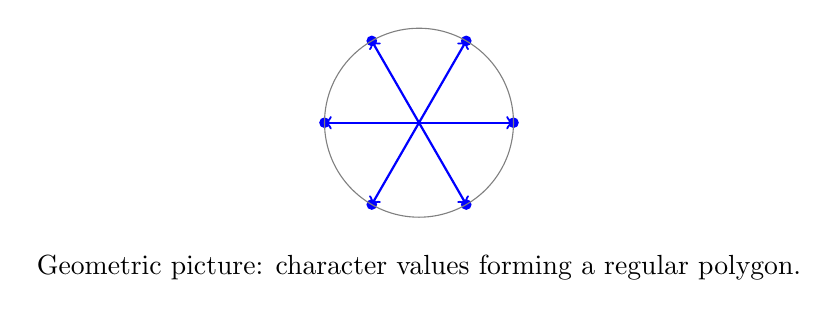
\begin{tikzpicture}[scale=1.2]
\foreach \x in {0,60,...,300}{
  \draw[thick,->,blue] (0,0)--(\x:1);
  \filldraw[blue] (\x:1) circle (0.05);
}
\draw[gray] (0,0) circle (1);
\node[below] at (0,-1.3){Geometric picture: character values forming a regular polygon.};
\end{tikzpicture}
\end{center}

% =====================================================
\section{Dual Group and Fourier Analysis}

\begin{definition}[Dual Group]\label{def:dual_group}
For a finite abelian group $G$, its \emph{dual group} is
\[
\widehat{G} = \mathrm{Hom}(G, \mathbb{C}^\times),
\]
the group of all complex-valued characters of $G$ under pointwise multiplication.
\end{definition}

\begin{definition}[Double Dual and Evaluation Map]\label{def:double_dual}
The \emph{double dual} of $G$ is
\[
\widehat{\widehat{G}} = \mathrm{Hom}(\widehat{G}, \mathbb{C}^\times).
\]
Define the \emph{evaluation map}
\[
\Phi: G \longrightarrow \widehat{\widehat{G}}, \qquad
(\Phi(g))(\chi) = \chi(g), \quad \forall g\in G,\,\chi\in\widehat{G}.
\]
\end{definition}

\begin{theorem}[Pontryagin Duality for Finite Abelian Groups]\label{thm:pontryagin}
The evaluation map $\Phi:G\to\widehat{\widehat{G}}$ is an isomorphism of groups.
\end{theorem}

\begin{proof}
We check injectivity and surjectivity.

\smallskip
\noindent\textbf{Injectivity.}
If $\Phi(g)=1$, then $\chi(g)=1$ for all $\chi\in\widehat{G}$.  
In a finite abelian group, characters \emph{separate points}: for every $g\ne e$, there exists $\chi$ with $\chi(g)\ne1$.  
Hence $\Phi(g)=1$ implies $g=e$, so $\Phi$ is injective.

\smallskip
\noindent\textbf{Cardinality equality.}
If $G\cong\mathbb{Z}_{n_1}\times\cdots\times\mathbb{Z}_{n_r}$,  
then each cyclic factor contributes $n_i$ characters, so
\[
|\widehat{G}|=n_1\cdots n_r=|G|.
\]
\smallskip
\noindent Since $\Phi$ is injective and $|G|=|\widehat{G}|$, it follows that $\Phi$ is bijective, hence an isomorphism.
\end{proof}

\begin{remark}
This is the finite version of Pontryagin duality, which extends to locally compact abelian groups in harmonic analysis.
\end{remark}

% -----------------------------------------------------
\subsection{Fourier Transform on Finite Abelian Groups}

\begin{definition}[Discrete Fourier Transform]\label{def:fourier}
Let $f:G\to\mathbb{C}$ be any function.  
Its \emph{Fourier transform} is the function $\widehat{f}:\widehat{G}\to\mathbb{C}$ defined by
\[
\widehat{f}(\chi)=\frac{1}{|G|}\sum_{g\in G} f(g)\overline{\chi(g)}.
\]
The inversion formula is
\[
f(g)=\sum_{\chi\in\widehat{G}}\widehat{f}(\chi)\chi(g).
\]
\end{definition}

\begin{proof}[Sketch of proof]
Multiply both sides by $\overline{\psi(g)}$ and sum over $g\in G$:
\[
\sum_{g\in G}f(g)\overline{\psi(g)} 
= \sum_{\chi\in\widehat{G}}\widehat{f}(\chi)\sum_{g\in G}\chi(g)\overline{\psi(g)}.
\]
By orthogonality (\Cref{thm:orthogonality}), only the term $\chi=\psi$ remains, giving $\widehat{f}(\psi)$.  
Hence the inversion formula holds.
\end{proof}

\begin{remark}
The characters $\chi\in\widehat{G}$ form an orthonormal basis of $\mathbb{C}[G]$ with respect to the inner product
\[
\langle f,h\rangle = \frac{1}{|G|}\sum_{g\in G} f(g)\,\overline{h(g)}.
\]
The Fourier transform changes from the \emph{group basis} $\{\delta_g\}$ to the \emph{character basis} $\{\chi\}$.
\end{remark}

\begin{corollary}[Double Fourier Transform]
Applying the transform twice yields
\[
\widehat{\widehat{f}}(g) = f(g^{-1}), \qquad g\in G.
\]
This mirrors the canonical isomorphism $G\cong\widehat{\widehat{G}}$ in \Cref{thm:pontryagin}.
\end{corollary}

% =====================================================
\section{Summary and Geometric Insight}

\begin{itemize}
    \item One-dimensional representations of a group $G$ are its \emph{characters}.
    \item The set of all characters $\widehat{G}$ forms the dual group, isomorphic to $G$ when $G$ is finite abelian.
    \item Nontrivial characters have vanishing sum and pairwise orthogonality.
    \item The discrete Fourier transform on $G$ expresses functions as linear combinations of characters.
\end{itemize}

\begin{center}
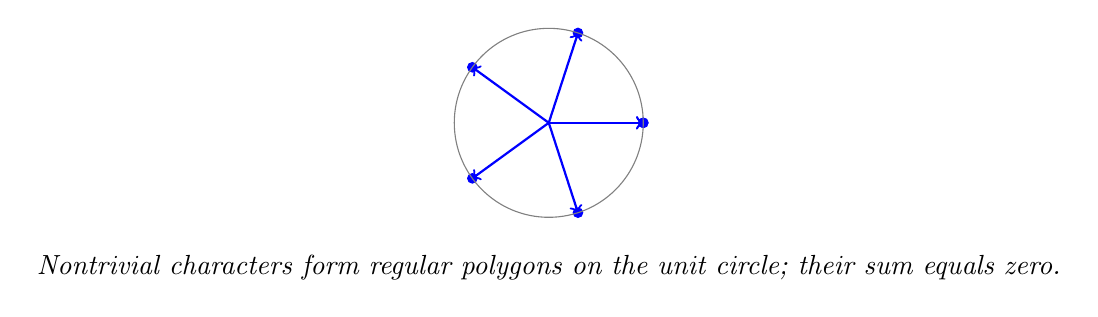
\begin{tikzpicture}[scale=1.2]
\foreach \x in {0,72,...,360}{
  \draw[thick,->,blue] (0,0)--(\x:1);
  \filldraw[blue] (\x:1) circle (0.05);
}
\draw[gray] (0,0) circle (1);
\node[below] at (0,-1.3)
{\textit{Nontrivial characters form regular polygons on the unit circle; their sum equals zero.}};
\end{tikzpicture}
\end{center}

\begin{proposition}
Let $K$ be a field, let $R$ be a unital $K$-algebra, and let $I\lhd R$ be a two-sided ideal.
Then the multiplication of $R$ descends to a well-defined $K$-bilinear map
\[
\overline{\mu}:\ (R/I)\times(R/I)\longrightarrow R/I,\qquad
(x+I,\ y+I)\longmapsto xy+I,
\]
which makes $R/I$ into a (unital) $K$-algebra.
\end{proposition}

\begin{proof}
\textbf{(1) $K$-vector space structure.}
Since $I$ is a $K$-linear subspace of $R$ (every ideal in a $K$-algebra is a $K$-subspace),
the quotient $R/I$ inherits a $K$-vector space structure with
\[
(x+I)+(y+I)=(x+y)+I,\qquad
\lambda\,(x+I)=(\lambda x)+I.
\]

\smallskip
\textbf{(2) Well-definedness of multiplication.}
Define $\overline{\mu}(x+I,\,y+I):=xy+I$.
Suppose $x'\equiv x\pmod I$ and $y'\equiv y\pmod I$, i.e.\ $x'=x+i_1$, $y'=y+i_2$ with $i_1,i_2\in I$.
Then
\[
x'y'=(x+i_1)(y+i_2)=xy + x i_2 + i_1 y + i_1 i_2.
\]
Because $I$ is a two-sided ideal, $x i_2\in I$, $i_1 y\in I$, and $i_1 i_2\in I$.
Hence $x'y'\equiv xy\pmod I$, so $x'y'+I=xy+I$.
Thus $\overline{\mu}$ is well defined.

\smallskip
\textbf{(3) $K$-bilinearity.}
For $\lambda\in K$ and $x,y,y_1,y_2\in R$,
\[
\overline{\mu}(x+I,\ (y_1+y_2)+I)
= x(y_1+y_2)+I
= (xy_1+I)+(xy_2+I)
= \overline{\mu}(x+I,y_1+I)+\overline{\mu}(x+I,y_2+I),
\]
\[
\overline{\mu}(x+I,\ \lambda y+I)
= x(\lambda y)+I
= \lambda(xy)+I
= \lambda\,\overline{\mu}(x+I,y+I).
\]
Similarly in the first argument:
\[
\overline{\mu}((x_1+x_2)+I,\ y+I)
= (x_1+x_2)y+I
= \overline{\mu}(x_1+I,y+I)+\overline{\mu}(x_2+I,y+I),
\]
\[
\overline{\mu}(\lambda x+I,\ y+I)
= (\lambda x)y+I
= \lambda(xy)+I
= \lambda\,\overline{\mu}(x+I,y+I).
\]
Hence $\overline{\mu}$ is $K$-bilinear.

\smallskip
\textbf{(4) Ring axioms.}
Associativity and distributivity descend from $R$:
for $x,y,z\in R$,
\[
\overline{\mu}\bigl(\overline{\mu}(x+I,y+I),z+I\bigr)
=(xy)z+I
= x(yz)+I
= \overline{\mu}\bigl(x+I,\ \overline{\mu}(y+I,z+I)\bigr).
\]
Distributivity over addition holds by bilinearity already checked.

\smallskip
\textbf{(5) Unit.}
If $1_R\notin I$, then $1_{R/I}:=1_R+I$ satisfies
\[
(1_R+I)(x+I)=x+I=(x+I)(1_R+I),
\]
so $R/I$ is unital. (If $1_R\in I$, then $R/I=0$ is the zero $K$-algebra, which is also unital only in the trivial sense.)

\smallskip
Altogether, $(R/I,\ \overline{\mu})$ is a $K$-algebra, and the canonical projection
$\pi:R\to R/I$ is a surjective homomorphism of $K$-algebras.
\end{proof}

\begin{remark}[Universal property]
If $\varphi:R\to A$ is a $K$-algebra homomorphism with $I\subseteq\ker\varphi$, there exists a unique $K$-algebra homomorphism
$\overline{\varphi}:R/I\to A$ such that $\varphi=\overline{\varphi}\circ\pi$.
Thus $R/I$ is the \emph{quotient $K$-algebra} of $R$ by $I$.
\end{remark}

\begin{proposition}[Polynomial and Free Algebras]\label{prop:poly-free}
\leavevmode
\begin{enumerate}
    \item The polynomial algebra
    \[
    K[x_1,\dots,x_n]
    \]
    is an infinite-dimensional commutative unital $K$-algebra.  
    Every finitely generated \emph{commutative} $K$-algebra is a quotient of a polynomial algebra by one of its ideals.

    \item The free (noncommutative) algebra
    \[
    K\langle x_1,\dots,x_n\rangle
    \]
    is an infinite-dimensional unital $K$-algebra which is generally noncommutative.  
    Every finitely generated (not necessarily commutative) $K$-algebra is a quotient of such a free algebra by a \emph{two-sided} ideal.
\end{enumerate}
\end{proposition}

\begin{proof}
\textbf{(i) Polynomial algebra.}
Let $K[x_1,\dots,x_n]$ denote the ring of polynomials in commuting indeterminates $x_1,\dots,x_n$ over the field $K$.
\begin{itemize}
    \item The multiplication and addition are the usual polynomial operations, both $K$-bilinear and associative.
    \item The identity element is $1\in K$.
    \item Since the monomials $x_1^{a_1}\cdots x_n^{a_n}$ with $(a_1,\dots,a_n)\in\mathbb{N}^n$ form a $K$-basis, the dimension of $K[x_1,\dots,x_n]$ over $K$ is infinite whenever $n\ge1$.
\end{itemize}
If $A$ is any finitely generated commutative $K$-algebra, say generated by elements $a_1,\dots,a_n\in A$, there exists a surjective $K$-algebra homomorphism
\[
\varphi:K[x_1,\dots,x_n]\longrightarrow A,\qquad x_i\longmapsto a_i.
\]
The kernel $\ker\varphi$ is an ideal of $K[x_1,\dots,x_n]$, and by the first isomorphism theorem,
\[
A\cong K[x_1,\dots,x_n]/\ker\varphi.
\]
Thus every finitely generated commutative $K$-algebra is a quotient of a polynomial algebra by an ideal.

\smallskip
\textbf{(ii) Free algebra.}
The \emph{free algebra} $K\langle x_1,\dots,x_n\rangle$ is the $K$-vector space having as basis all finite words (monomials)
\[
1,\ x_i,\ x_ix_j,\ x_ix_jx_k,\ \dots
\]
in the noncommuting symbols $x_1,\dots,x_n$, with multiplication given by concatenation of words and extended $K$-bilinearly.  
Explicitly, if $u,v$ are two words, then $u\cdot v$ is their concatenation.

\begin{itemize}
    \item The product is associative and $K$-bilinear, and the unit element is the empty word $1$.
    \item The dimension of $K\langle x_1,\dots,x_n\rangle$ over $K$ is infinite since it has one basis element for every word of any finite length.
    \item The algebra is noncommutative as soon as $n\ge2$, since $x_1x_2\ne x_2x_1$.
\end{itemize}

Now let $A$ be a finitely generated (possibly noncommutative) $K$-algebra with generators $a_1,\dots,a_n$.  
Define a surjective homomorphism
\[
\Phi:K\langle x_1,\dots,x_n\rangle\longrightarrow A,\qquad x_i\longmapsto a_i.
\]
Its kernel $\ker\Phi$ is a \emph{two-sided} ideal of $K\langle x_1,\dots,x_n\rangle$, and again by the isomorphism theorem,
\[
A\cong K\langle x_1,\dots,x_n\rangle/\ker\Phi.
\]
Thus every finitely generated $K$-algebra arises as a quotient of the free algebra by a two-sided ideal.
\end{proof}

\begin{remark}
The polynomial algebra $K[x_1,\dots,x_n]$ can be obtained from the free algebra $K\langle x_1,\dots,x_n\rangle$ by imposing commutativity relations:
\[
K[x_1,\dots,x_n]\ \cong\ K\langle x_1,\dots,x_n\rangle/\bigl(x_ix_j-x_jx_i\mid 1\le i,j\le n\bigr).
\]
Hence the free algebra plays the same universal role for noncommutative algebras that the polynomial algebra does for commutative ones.
\end{remark}

\begin{definition}[K-algebra homomorphism]
A \emph{$K$-algebra homomorphism} is a homomorphism of rings that is also $K$-linear.  
In other words, if $R$ and $S$ are $K$-algebras, a map $\varphi:R\to S$ is a $K$-algebra homomorphism if:
\[
\varphi(x+y)=\varphi(x)+\varphi(y),\quad
\varphi(xy)=\varphi(x)\varphi(y),\quad
\]
\[
\varphi(1_R)=1_S,\quad
\varphi(a x)=a\,\varphi(x)\ \text{for all }a\in K,\ x,y\in R.
\]
\end{definition}

\begin{remark}
Thus a $K$-algebra homomorphism preserves both the ring operations and the scalar multiplication by elements of $K$.
\end{remark}

% -----------------------------------------------------
\begin{definition}[Module over a $K$-algebra {\normalfont(Definition 1.1.12)}]\label{def:module_K-algebra}
Let $R$ be a $K$-algebra.  
An \emph{$R$-module} is a pair $(\tilde{\rho},V)$ where:
\begin{itemize}
    \item $V$ is a $K$-vector space, and
    \item $\tilde{\rho}:R\to \mathrm{End}_K(V)$ is a $K$-algebra homomorphism.
\end{itemize}
We always assume that $\tilde{\rho}$ sends the unit of $R$ to the unit of $\mathrm{End}_K(V)$:
\[
\tilde{\rho}(1_R)=\mathrm{id}_V.
\]
Such modules are called \emph{unital modules}.
\end{definition}

\begin{remark}
The notion of an $R$-module given above requires $\tilde{\rho}$ to be $K$-linear and is therefore slightly stronger than the general definition of a module for a ring (see, for instance, \emph{[1, Chapter 12, Section 1]}).  
This definition, however, is precisely what is needed to establish the correspondence between group representations of a group $G$ and modules over the \emph{group algebra} $K[G]$ associated with $G$.
\end{remark}

% -----------------------------------------------------
\begin{example}[Left ideals and submodules {\normalfont(Example 1.1.13)}]\label{ex:leftideal_module}
Every left ideal $I$ of a $K$-algebra $R$ is naturally an $R$-module under the multiplication action
\[
r\cdot x = r x, \qquad \text{for all } r\in R,\ x\in I.
\]
Moreover:
\begin{itemize}
    \item Any subspace $N$ of an $R$-module $M$ that is closed under the $R$-action
    (that is, $r\cdot n\in N$ for all $r\in R$, $n\in N$)
    is called a \emph{submodule}.
    \item The quotient space $M/N$ inherits an induced $R$-action
    \[
    r\cdot(m+N) = (r\cdot m) + N,
    \]
    making $M/N$ again an $R$-module.
\end{itemize}
\end{example}

% -----------------------------------------------------
\begin{example}[Matrix module {\normalfont(Example 1.1.14)}]\label{ex:MnK-module}
Let $R = M_n(K)$ be the algebra of $n\times n$ matrices over $K$.  
Then the vector space $K^n$ becomes an $R$-module by defining the action
\[
A\cdot v = A v,
\]
where $v\in K^n$ is viewed as a column vector and $A\in M_n(K)$ acts by matrix multiplication on the left.

The corresponding $K$-algebra homomorphism is
\[
\tilde{\rho}: M_n(K)\longrightarrow \mathrm{End}_K(K^n), \quad A\longmapsto (v\mapsto Av),
\]
which is injective, unital, and $K$-linear.
\end{example}

% -----------------------------------------------------
\begin{definition}[Group algebra]\label{def:group_algebra}
Let $G$ be a group.  
The \emph{group algebra} $K[G]$ of $G$ over a field $K$ is defined as follows:
\begin{itemize}
    \item As a vector space, $K[G]$ is the free $K$-vector space with basis
    \[
    \{\,1_g \mid g\in G\,\}.
    \]
    \item Multiplication is defined by extending linearly the group law of $G$:
    \[
    1_g\,1_h = 1_{gh}, \qquad \forall\, g,h\in G.
    \]
\end{itemize}
\end{definition}

\begin{remark}
Every element of $K[G]$ can be written uniquely as a finite linear combination
\[
\sum_{g\in G} a_g\,1_g,\quad a_g\in K,
\]
and multiplication extends bilinearly according to the group product:
\[
\left(\sum_g a_g 1_g\right)\!\left(\sum_h b_h 1_h\right)
= \sum_{g,h} a_g b_h\,1_{gh}.
\]
Then $K[G]$ is a unital, associative, and \emph{commutative} $K$-algebra if and only if $G$ is abelian.
\end{remark}

\begin{remark}[Group algebra as a function algebra]\label{rem:group-algebra-convolution}
Another useful way to view the group algebra $K[G]$ is as the algebra of $K$-valued functions on $G$
whose multiplication is given by \emph{convolution}.

Let
\[
\mathrm{Fun}(G,K)=\{\,f:G\to K\,\}
\]
be the $K$-vector space of all functions from $G$ to $K$ (or the space of finitely supported functions if $G$ is infinite).

For $f_1,f_2\in\mathrm{Fun}(G,K)$, define their \emph{convolution product}
\[
(f_1*f_2)(g)
   \;=\;
   \sum_{\substack{x,y\in G\\ xy=g}} f_1(x)\,f_2(y),
   \qquad g\in G.
\]
The sum is finite if $G$ is finite or if the functions have finite support.

Then $\mathrm{Fun}(G,K)$, equipped with pointwise addition, scalar multiplication, and this convolution product, becomes a (generally noncommutative) $K$-algebra.
\end{remark}

% -----------------------------------------------------
% -----------------------------------------------------
\begin{exercise}[1.1.15]\label{ex:1.1.15}
Identify the basis element $1_g\in K[G]$ with the function
\[
\delta_g:G\longrightarrow K, \qquad
\delta_g(h)=
\begin{cases}
1, & \text{if } h=g,\\[4pt]
0, & \text{otherwise.}
\end{cases}
\]
Show that, under this identification, the multiplication in $K[G]$ corresponds exactly
to the convolution of functions on $G$.
\end{exercise}

\begin{proof}
We recall that the group algebra $K[G]$ has basis $\{1_g\mid g\in G\}$ with product defined by
\[
1_g\,1_h = 1_{gh}, \qquad g,h\in G.
\]
Meanwhile, the algebra of $K$-valued functions on $G$ has multiplication given by the
\emph{convolution product}:
\[
(f_1 * f_2)(z)
   = \sum_{\substack{x,y\in G\\ xy=z}} f_1(x)f_2(y)
   = \sum_{x\in G} f_1(x)f_2(x^{-1}z),
   \qquad z\in G.
\]

\smallskip
\noindent
\textbf{Step 1. Convolution of delta functions.}
Let $f_1=\delta_g$ and $f_2=\delta_h$.
Then for each $z\in G$,
\[
(\delta_g*\delta_h)(z)
   = \sum_{xy=z}\delta_g(x)\,\delta_h(y).
\]
The product $\delta_g(x)\delta_h(y)$ is nonzero only when $x=g$ and $y=h$,
and in that case $xy=gh$.
Hence
\[
(\delta_g*\delta_h)(z)
   =
   \begin{cases}
      1, & \text{if } z=gh,\\[4pt]
      0, & \text{otherwise.}
   \end{cases}
   = \delta_{gh}(z).
\]

\smallskip
\noindent
\textbf{Step 2. Identification with the group algebra.}
Under the identification $1_g\leftrightarrow \delta_g$, the convolution product satisfies
\[
\delta_g*\delta_h = \delta_{gh}
\quad\Longleftrightarrow\quad
1_g\,1_h = 1_{gh}.
\]
Therefore, the convolution algebra of finitely supported functions $f:G\to K$
is \emph{isomorphic} to the group algebra $K[G]$ as a $K$-algebra.

\smallskip
\noindent
\textbf{Conclusion.}
The correspondence
\[
1_g \;\longleftrightarrow\; \delta_g
\]
is a $K$-linear bijection that preserves multiplication (convolution),
hence establishes an isomorphism of $K$-algebras:
\[
K[G] \;\cong\;
\bigl\{f:G\to K\bigr\}, \qquad
(f_1,f_2)\longmapsto f_1*f_2.
\]
\end{proof}

% -----------------------------------------------------
\begin{exercise}[1.1.16]\label{ex:1.1.16}
Let $n>1$ be an integer and $G=\mathbb{Z}/n\mathbb{Z}=\{0,1,\dots,n-1\}$.
Show that the group algebra $K[\mathbb{Z}/n\mathbb{Z}]$ is isomorphic, as a $K$-algebra, to the quotient ring
\[
K[t]/(t^n-1),
\]
where $(t^n-1)$ denotes the ideal in $K[t]$ generated by $t^n-1$.
\end{exercise}

\begin{proof}[Solution sketch]
Let $g$ denote the generator of the cyclic group $\mathbb{Z}/n\mathbb{Z}$.
Then every element of $K[G]$ can be written as a $K$-linear combination
\[
a_0\,1_{g^0}+a_1\,1_{g^1}+\cdots+a_{n-1}\,1_{g^{n-1}},\quad a_i\in K,
\]
and the multiplication rule satisfies $1_{g^i}1_{g^j}=1_{g^{i+j}}$ with indices taken mod~$n$.

Define a $K$-algebra homomorphism
\[
\Phi:K[t]\longrightarrow K[G],
\qquad \Phi(t)=1_g.
\]
Then $\Phi(t^n-1)=1_{g^n}-1_e=1_e-1_e=0$, so $(t^n-1)\subseteq\ker\Phi$.  
Hence $\Phi$ induces a surjective homomorphism
\[
\overline{\Phi}:K[t]/(t^n-1)\twoheadrightarrow K[G].
\]
Both algebras are $n$-dimensional $K$-vector spaces with bases
\[
\{\,t^0,t^1,\dots,t^{n-1}\,\} \quad\text{and}\quad \{\,1_{g^0},1_{g^1},\dots,1_{g^{n-1}}\,\},
\]
so $\overline{\Phi}$ is an isomorphism.
Thus $K[\mathbb{Z}/n\mathbb{Z}]\cong K[t]/(t^n-1)$ as $K$-algebras.
\end{proof}

% =====================================================
\section{Representations and Modules over the Group Algebra}

\begin{theorem}\label{thm:representation_KG-module}
Let $G$ be a group and $K$ a field.
\begin{enumerate}
    \item If $\rho:G\to GL(V)$ is a representation of $G$ on a finite-dimensional $K$-vector space $V$, then there exists a unique $K$-algebra homomorphism
    \[
    \tilde{\rho}:K[G]\longrightarrow \mathrm{End}_K(V)
    \]
    defined by
    \begin{equation}\label{eq:rho-tilde-def}
        \tilde{\rho}(f) = \sum_{g\in G} f(g)\,\rho(g), \qquad f\in K[G].
    \end{equation}
    This makes $(\tilde{\rho},V)$ a unital $K[G]$-module.

    \item Conversely, if $(\tilde{\rho},V)$ is a unital $K[G]$-module, then defining
    \begin{equation}\label{eq:rho-from-tilde}
        \rho(g) := \tilde{\rho}(1_g), \qquad g\in G,
    \end{equation}
    yields a group representation $\rho:G\to GL(V)$.

    \item The constructions \eqref{eq:rho-tilde-def} and \eqref{eq:rho-from-tilde} are mutually inverse, giving a one-to-one correspondence between representations of $G$ over $K$ and unital $K[G]$-modules.
\end{enumerate}
\end{theorem}

\begin{proof}
\textbf{(i) From representation to module.}
Let $\rho:G\to GL(V)$ be a representation.
Define $\tilde{\rho}$ by linear extension from $G$ to $K[G]$:
\[
\tilde{\rho}\!\left(\sum_{g\in G} a_g\,1_g\right)
  = \sum_{g\in G} a_g\,\rho(g), \qquad a_g\in K.
\]
Since $\rho(gh)=\rho(g)\rho(h)$, we compute for $f_1,f_2\in K[G]$:
\[
\tilde{\rho}(f_1f_2)
 = \tilde{\rho}\!\left(\sum_{x,y} f_1(x)f_2(y)\,1_{xy}\right)
 = \sum_{x,y} f_1(x)f_2(y)\rho(xy)
 = \left(\sum_x f_1(x)\rho(x)\right)\!\left(\sum_y f_2(y)\rho(y)\right)
 = \tilde{\rho}(f_1)\tilde{\rho}(f_2).
\]
Thus $\tilde{\rho}$ is a $K$-algebra homomorphism.  
Moreover, $\tilde{\rho}(1_e)=\rho(e)=\mathrm{id}_V$, so the module is unital.

\smallskip
\textbf{(ii) From module to representation.}
Conversely, let $\tilde{\rho}:K[G]\to \mathrm{End}_K(V)$ be a $K$-algebra homomorphism with $\tilde{\rho}(1_e)=\mathrm{id}_V$.  
Define $\rho(g)=\tilde{\rho}(1_g)$.  
Then
\[
\rho(g)\rho(h)
 = \tilde{\rho}(1_g)\tilde{\rho}(1_h)
 = \tilde{\rho}(1_g1_h)
 = \tilde{\rho}(1_{gh})
 = \rho(gh).
\]
Also $\rho(e)=\tilde{\rho}(1_e)=\mathrm{id}_V$, and $\rho(g)$ is invertible with inverse $\rho(g^{-1})$, since
\[
\rho(g)\rho(g^{-1})=\tilde{\rho}(1_e)=\mathrm{id}_V.
\]
Hence $\rho:G\to GL(V)$ is a group representation.

\smallskip
\textbf{(iii) Mutual inverses.}
The constructions \eqref{eq:rho-tilde-def} and \eqref{eq:rho-from-tilde} clearly invert each other:
\[
\tilde{\rho}(1_g) = \rho(g),\qquad
\rho(g) \mapsto \tilde{\rho}(1_g),
\]
so there is a natural equivalence between the category of representations of $G$ over $K$ and the category of unital $K[G]$-modules.
\end{proof}

\begin{remark}
This correspondence allows the use of ring- and module-theoretic tools in studying representations of groups.
The representation $\rho$ can be thought of as the restriction of the $K[G]$-module structure on $V$ to the subgroup $G\subseteq K[G]^\times$.
\end{remark}

% -----------------------------------------------------
\begin{example}[Regular representations {\normalfont(Example 1.1.17)}]\label{ex:regular_representation}
Let $R$ be a $K$-algebra.  
For each $r\in R$, define a $K$-linear map
\[
\tilde{L}(r):R\longrightarrow R,\qquad \tilde{L}(r)(x)=r x,
\]
that is, left multiplication by $r$.  
This defines a $K$-algebra homomorphism
\[
\tilde{L}:R\longrightarrow \mathrm{End}_K(R),
\]
making $R$ into a left $R$-module called the \emph{left regular module}.

\medskip
Now let $R=K[G]$ be the group algebra.  
Then for each $g\in G$, define
\[
L(g):K[G]\to K[G], \qquad L(g)(1_x)=1_{gx}.
\]
This gives a representation $L:G\to GL(K[G])$, called the \emph{left regular representation} of $G$.

\smallskip
Similarly, defining
\[
R(g):K[G]\to K[G], \qquad R(g)(1_x)=1_{xg^{-1}},
\]
yields another representation $R:G\to GL(K[G])$, called the \emph{right regular representation}.
\end{example}

% -----------------------------------------------------
% -----------------------------------------------------
\begin{exercise}[1.1.18]\label{ex:1.1.18}
If $K[G]$ is viewed as the algebra of $K$-valued functions on $G$
(as in Exercise~\ref{ex:1.1.15}),
then the left and right regular representations act by
\[
(L(g)f)(x)=f(g^{-1}x),
\qquad
(R(g)f)(x)=f(xg),
\]
for all $f:G\to K$ and $g,x\in G$.
\end{exercise}

\begin{proof}
We use the basis $\{1_y\mid y\in G\}$ of $K[G]$ and recall that the left and right regular actions are defined by
\[
L(g)\,1_y = 1_{gy},
\qquad
R(g)\,1_y = 1_{y g^{-1}},
\qquad g,y\in G.
\]

\smallskip
\noindent\textbf{Step 1. Left regular action.}
Let $f=\sum_{y\in G} f(y)\,1_y \in K[G]$.
Then
\[
L(g)f
   = L(g)\!\left(\sum_{y\in G} f(y)\,1_y\right)
   = \sum_{y\in G} f(y)\,L(g)(1_y)
   = \sum_{y\in G} f(y)\,1_{gy}.
\]
To find the coefficient of $1_x$ in $L(g)f$, observe that
$1_{gy}=1_x$ precisely when $y=g^{-1}x$.
Hence the coefficient of $1_x$ equals $f(g^{-1}x)$.
Identifying $1_x$ with the delta function $\delta_x$ as in
Exercise~\ref{ex:1.1.15}, this means that
\[
(L(g)f)(x) = f(g^{-1}x),
\]
which is the claimed formula for the left regular representation.

\smallskip
\noindent\textbf{Step 2. Right regular action.}
Similarly,
\[
R(g)f
   = R(g)\!\left(\sum_{y\in G} f(y)\,1_y\right)
   = \sum_{y\in G} f(y)\,R(g)(1_y)
   = \sum_{y\in G} f(y)\,1_{y g^{-1}}.
\]
Now $1_{y g^{-1}}=1_x$ if and only if $y=xg$,
so the coefficient of $1_x$ equals $f(xg)$.
Thus
\[
(R(g)f)(x) = f(xg).
\]

\smallskip
\noindent\textbf{Step 3. Conclusion.}
Under the identification $K[G]\cong\{f:G\to K\}$,
the left and right regular representations act by the explicit formulas:
\[
(L(g)f)(x)=f(g^{-1}x),
\qquad
(R(g)f)(x)=f(xg).
\]
These describe, respectively, the \emph{left translation} and \emph{right translation}
actions of $G$ on the space of $K$-valued functions on $G$.
\end{proof}

\begin{remark}
The formulas above show that $L(g)$ and $R(g)$ commute for all $g\in G$:
\[
L(g)\,R(h) = R(h)\,L(g), \qquad \forall\, g,h\in G,
\]
since
\[
(L(g)R(h)f)(x)=f(g^{-1}xh)=(R(h)L(g)f)(x).
\]
Thus the left and right regular representations yield commuting actions of $G$
on $K[G]$.
\end{remark}


% =====================================================
\section{Invariant Subspaces and Simplicity}\label{sec:invariant-simplicity}

\begin{definition}[Invariant subspace {\normalfont(Definition 1.2.1)}]\label{def:invariant-subspace}
Let $\rho:G\to GL(V)$ be a representation of a group $G$ over a field $K$.

A subspace $W\subseteq V$ is called an \emph{invariant subspace} (or \emph{subrepresentation}) if
\[
\rho(g)W \subseteq W, \qquad \forall\, g\in G.
\]
Equivalently, for every $w\in W$ and every $g\in G$, the vector $\rho(g)w$ also lies in $W$.

\smallskip
Similarly, if $(\tilde{\rho},V)$ is an $R$-module, where $\tilde{\rho}:R\to\End_K(V)$ is a $K$-algebra homomorphism,
then a subspace $W\subseteq V$ is called \emph{invariant} (or a \emph{submodule}) if
\[
\tilde{\rho}(r)W\subseteq W, \qquad \forall\, r\in R.
\]
\end{definition}

\begin{remark}
An invariant subspace of a representation is often called a \emph{subrepresentation}, while an invariant subspace of a module is called a \emph{submodule}.
\end{remark}

% -----------------------------------------------------
\begin{example}[Invariant subspaces in the regular representation {\normalfont(Example 1.2.2)}]\label{ex:regular-invariants}
Consider the left regular representation $(L,K[G])$, where $L(g):K[G]\to K[G]$ acts by
\[
L(g)(1_x)=1_{gx}, \qquad g,x\in G.
\]

\begin{itemize}
    \item The subspace of constant functions
    \[
    W_{\mathrm{const}}=\{\,f:G\to K \mid f(g)=c \text{ for some } c\in K\,\}
    \]
    is one-dimensional and invariant, since $(L(g)f)(x)=f(g^{-1}x)=c$ for all $x,g\in G$.

    \item The subspace
    \[
    K[G]^0=\Bigl\{\,f:G\to K \ \Bigm|\  \sum_{g\in G}f(g)=0\,\Bigr\}
    \]
    consists of functions whose total sum over $G$ is zero.
    It has dimension $|G|-1$ and is also invariant under $L(g)$, since
    \[
    \sum_{x\in G}(L(g)f)(x)
      = \sum_{x} f(g^{-1}x)
      = \sum_{y} f(y)
      = 0.
    \]
\end{itemize}
\end{example}

% -----------------------------------------------------
\begin{exercise}[1.2.3]\label{ex:1.2.3}
Show that the subspace $K[G]^0$ defined in Example~\ref{ex:regular-invariants}
has an invariant complement in $(L,K[G])$ if and only if $|G|$ is not divisible by the characteristic of $K$
(in particular, this always holds if $\mathrm{char}(K)=0$).
\end{exercise}

\begin{proof}
Let
\[
W_{\mathrm{const}}=\{\,f:G\to K \mid f(g)=c \text{ for some constant } c\in K\,\}
\]
be the one-dimensional subspace of constant functions in $K[G]$.
We have already seen that $W_{\mathrm{const}}$ is invariant under the left regular action
\[
(L(g)f)(x)=f(g^{-1}x), \qquad g,x\in G.
\]

We seek an invariant complement to $W_{\mathrm{const}}$,
that is, an invariant subspace $U$ such that
\[
K[G]=W_{\mathrm{const}}\oplus U.
\]
We claim that $U=K[G]^0$ serves this role if and only if $|G|$ is invertible in $K$.

\medskip
\noindent\textbf{Step 1. Construction of the projection.}
Define the $K$-linear map
\[
P:K[G]\longrightarrow W_{\mathrm{const}},\qquad
P(f)=\frac{1}{|G|}\sum_{g\in G} f(g).
\]
Here $P(f)$ is the constant function on $G$ with value equal to the average of $f$ over $G$.
The scalar $\tfrac{1}{|G|}$ is meaningful only if $|G|$ is invertible in $K$ (that is, if $\mathrm{char}(K)\nmid |G|$).

\medskip
\noindent\textbf{Step 2. $G$-equivariance of $P$.}
For $h\in G$,
\[
(P\circ L(h))(f)
  = \frac{1}{|G|}\sum_{x\in G}(L(h)f)(x)
  = \frac{1}{|G|}\sum_{x} f(h^{-1}x)
  = \frac{1}{|G|}\sum_{y\in G}f(y)
  = P(f),
\]
where we have substituted $y=h^{-1}x$.
Thus $P(L(h)f)=P(f)$ for all $h\in G$, i.e.\ $P$ is $G$-equivariant.

\medskip
\noindent\textbf{Step 3. Kernel and image.}
The image of $P$ is precisely $W_{\mathrm{const}}$.
Indeed, for any constant function $f(g)=c$, we have $P(f)=c$, so $\mathrm{im}\,P=W_{\mathrm{const}}$.
The kernel of $P$ is
\[
\ker P=\Bigl\{\,f:G\to K \ \Bigm|\  \sum_{g\in G}f(g)=0\,\Bigr\}=K[G]^0,
\]
and since $P$ is $G$-equivariant, $\ker P$ is an invariant subspace.

\medskip
\noindent\textbf{Step 4. Direct-sum decomposition.}
Because $P$ is a projection ($P^2=P$), we have
\[
K[G]=\ker P\oplus\mathrm{im}\,P
      =K[G]^0\oplus W_{\mathrm{const}}.
\]
Thus $K[G]^0$ is an invariant complement to $W_{\mathrm{const}}$.

\medskip
\noindent\textbf{Step 5. Necessity of the condition.}
If $\mathrm{char}(K)$ divides $|G|$, then $|G|=0$ in $K$ and the map $P$ above is not defined.
In that case, the only $G$-equivariant projection onto $W_{\mathrm{const}}$ is the zero map,
so no invariant complement exists.

\medskip
\noindent\textbf{Conclusion.}
Hence $K[G]^0$ has an invariant complement in $(L,K[G])$ if and only if $|G|$ is invertible in $K$,
that is, if and only if the characteristic of $K$ does not divide $|G|$.
\end{proof}


% -----------------------------------------------------
\begin{exercise}[1.2.4]\label{ex:1.2.4}
Let $G=\mathbb{Z}/2\mathbb{Z}=\{0,1\}$ and let $K$ be a field of characteristic two.
Show that the subspace of $K[G]$ spanned by $1_0+1_1$ is the only non-trivial proper invariant subspace
for the left (or right) regular representation of $G$.
\end{exercise}

\begin{proof}
The group algebra of $G$ is
\[
K[G]=K1_0\oplus K1_1,
\]
a two-dimensional $K$-vector space with basis $\{1_0,1_1\}$ and multiplication determined by
\[
1_0 1_0 = 1_0, \qquad
1_0 1_1 = 1_1, \qquad
1_1 1_0 = 1_1, \qquad
1_1 1_1 = 1_0,
\]
since addition in $G$ is modulo $2$.

\medskip
\noindent\textbf{Step 1. The left regular representation.}
The left regular action $L:G\to GL(K[G])$ is given by
\[
L(g)(1_h) = 1_{g+h}, \qquad g,h\in G.
\]
In particular,
\[
L(0)(1_0)=1_0, \quad L(0)(1_1)=1_1, \qquad
L(1)(1_0)=1_1, \quad L(1)(1_1)=1_0.
\]
Thus $L(1)$ \emph{interchanges} $1_0$ and $1_1$.

\medskip
\noindent\textbf{Step 2. Determine invariant subspaces.}
Let $W\subseteq K[G]$ be a subspace invariant under $L(1)$.
Write a general element as $v=a\,1_0+b\,1_1$ with $a,b\in K$.
Then
\[
L(1)v = a\,L(1)(1_0) + b\,L(1)(1_1) = a\,1_1 + b\,1_0.
\]
Hence invariance means that $L(1)v\in W$ whenever $v\in W$.

We check the possible one-dimensional subspaces \( W = K(\alpha 1_0 + \beta 1_1) \):
\[
L(1)(\alpha 1_0 + \beta 1_1) = \alpha 1_1 + \beta 1_0.
\]
For $W$ to be invariant, this vector must be a scalar multiple of $\alpha 1_0+\beta 1_1$.
That is, there must exist $\lambda\in K$ such that
\[
(\alpha 1_1 + \beta 1_0) = \lambda(\alpha 1_0 + \beta 1_1),
\]
or equivalently, comparing coefficients:
\[
\beta = \lambda\alpha, \qquad \alpha = \lambda\beta.
\]
If $\alpha\beta\ne0$, these imply $\lambda^2=1$.

\medskip
\noindent\textbf{Step 3. Effect of the characteristic.}
If $\mathrm{char}(K)\ne2$, the two solutions $\lambda=\pm1$ give two distinct invariant lines
\[
K(1_0+1_1), \qquad K(1_0-1_1).
\]
However, when $\mathrm{char}(K)=2$, the two coincide because
\[
1_0 - 1_1 = 1_0 + 1_1.
\]
Thus in characteristic two, there is only one non-trivial proper invariant subspace:
\[
W = K(1_0 + 1_1).
\]

\medskip
\noindent\textbf{Step 4. Right regular representation.}
The right regular representation $R(g)$ satisfies $R(1)(1_h)=1_{h+1}$, which also interchanges $1_0$ and $1_1$,
so the same argument applies.  
Hence $W=K(1_0+1_1)$ is also the only non-trivial invariant subspace for the right regular representation.

\medskip
\noindent\textbf{Conclusion.}
Therefore, over a field of characteristic two, the subspace spanned by $1_0+1_1$ is the unique non-trivial proper invariant subspace for both the left and right regular representations of $G$.
\end{proof}

% -----------------------------------------------------
\begin{exercise}[1.2.5]\label{ex:1.2.5}
Show that if every representation of a group $G$ is a direct sum of one-dimensional invariant subspaces,
then $G$ must be abelian.

\emph{Hint.} Apply this assumption to the regular representation $(L,K[G])$ and use that
distinct group elements act as linearly independent operators (cf.\ Exercise~1.1.4).
\end{exercise}

\begin{proof}
Assume that every (finite-dimensional) representation of $G$ over $K$ decomposes as a direct sum of
one-dimensional invariant subspaces. In particular, this holds for the \emph{left regular representation}
$L:G\to GL(K[G])$ given by $L(g)(1_x)=1_{gx}$.

\smallskip
\noindent\textbf{Step 1: Decomposition into $1$-dimensional subrepresentations.}
By hypothesis, there exists a direct-sum decomposition
\[
K[G] \;=\; V_1 \oplus \cdots \oplus V_m,
\]
where each $V_i$ is $1$-dimensional and $G$-invariant under $L$.  
Fix for each $i$ a nonzero vector $v_i\in V_i$.  
Since $V_i$ is $G$-invariant and $1$-dimensional, there is a \emph{character} $\chi_i:G\to K^\times$ such that
\[
L(g)v_i \;=\; \chi_i(g)\,v_i \qquad (\forall\,g\in G).
\]
Thus, with respect to the basis $\{v_1,\dots,v_m\}$, every $L(g)$ is a diagonal matrix:
\[
L(g) \;=\; \mathrm{diag}\big(\chi_1(g),\dots,\chi_m(g)\big).
\]

\smallskip
\noindent\textbf{Step 2: Commutativity of the image $L(G)$.}
Diagonal matrices with respect to the \emph{same} basis commute. Hence, for all $g,h\in G$,
\[
L(g)\,L(h) \;=\; L(h)\,L(g).
\]
Using $L$ is a homomorphism, this reads
\[
L(gh) \;=\; L(hg).
\]

\smallskip
\noindent\textbf{Step 3: Faithfulness of the regular representation.}
The left regular representation is faithful: if $L(g)=\mathrm{id}_{K[G]}$, then
\[
1_{gx} \;=\; L(g)(1_x) \;=\; 1_x \qquad (\forall\,x\in G),
\]
which forces $gx=x$ for all $x$, hence $g=e$. Therefore $\ker L=\{e\}$.

\smallskip
\noindent\textbf{Step 4: Conclusion.}
From $L(gh)=L(hg)$ and the injectivity of $L$, we conclude $gh=hg$ for all $g,h\in G$.  
Thus $G$ is abelian.
\end{proof}

\begin{remark}
A variant of Step~3 uses the fact (cf.\ Exercise~1.1.4) that the operators $\{L(g)\mid g\in G\}$ are linearly independent in
$\End_K(K[G])$. If $L(gh)=L(hg)$, then $L(gh-hg)=0$ and linear independence again yields $gh=hg$.
\end{remark}


% -----------------------------------------------------
\begin{definition}[Simplicity {\normalfont(Definition 1.2.6)}]\label{def:simple}
A representation $(\rho,V)$ of a group $G$ or, more generally, a module $(\tilde{\rho},V)$ over a $K$-algebra $R$
is said to be \emph{simple} (or \emph{irreducible}) if it has no non-trivial proper invariant subspaces:
\[
V\ne\{0\}, \quad\text{and if } W\subseteq V\text{ satisfies }\rho(g)W\subseteq W\ \forall g\in G,\text{ then }W=\{0\}\text{ or }W=V.
\]
By convention, the zero-dimensional representation (the trivial module $\{0\}$) is not considered simple.
\end{definition}

\begin{remark}
This convention is analogous to the number 1 not being regarded as a prime number.
\end{remark}

% -----------------------------------------------------
% -----------------------------------------------------
\begin{example}[Simple representations]\label{ex:simple-1D}
Every one-dimensional representation (or character) is simple,
since the only subspaces of a one-dimensional vector space are $\{0\}$ and the space itself.
\end{example}

% -----------------------------------------------------
\begin{exercise}[1.2.8]\label{ex:1.2.8}
Show that every simple module for a finite-dimensional $K$-algebra is finite-dimensional.
\end{exercise}

\begin{proof}
Let $A$ be a finite-dimensional $K$-algebra and $M$ a simple left $A$-module.

\smallskip
\noindent
\textbf{Step 1: Generation by a single element.}
Pick any nonzero $m\in M$.  
The subset
\[
A\cdot m = \{\,a m \mid a\in A\,\}
\]
is a submodule of $M$, since for any $b\in A$ and $a\in A$,
\[
b(a m) = (ba)m \in A\cdot m.
\]
Because $M$ is simple, $A\cdot m$ is nonzero and therefore equals $M$:
\[
M = A\cdot m.
\]
Thus $M$ is generated by a single element as an $A$-module.

\smallskip
\noindent
\textbf{Step 2: Finite-dimensionality.}
The map
\[
\varphi:A \longrightarrow M,\qquad \varphi(a)=a m
\]
is a surjective $K$-linear map.  
Hence,
\[
\dim_K(M) = \dim_K(A/\ker\varphi) \le \dim_K(A).
\]
Since $A$ is finite-dimensional over $K$, it follows that $M$ is finite-dimensional as well.

\smallskip
\noindent
\textbf{Conclusion.}
Every simple module over a finite-dimensional $K$-algebra is finite-dimensional.
\end{proof}

\begin{remark}
This argument shows more generally that any finitely generated module over a finite-dimensional
$K$-algebra is finite-dimensional, since each generator contributes at most $\dim_K(A)$ dimensions.
\end{remark}


% -----------------------------------------------------
% =====================================================
\begin{exercise}[1.2.9]\label{ex:1.2.9}
Suppose $K$ is algebraically closed and $G$ is abelian.
Show that every simple representation of $G$ over $K$ is one-dimensional.

\emph{Hint.}  
A commuting family of matrices over an algebraically closed field can be simultaneously
upper-triangularized. Deduce that any finite-dimensional representation of an abelian group
has a nonzero invariant one-dimensional subspace.
\end{exercise}

\begin{proof}
Let $\rho:G\to GL(V)$ be a finite-dimensional representation of the abelian group $G$
over an algebraically closed field $K$.
We must show that $\rho$ has a nonzero invariant one-dimensional subspace.
Equivalently, $V$ contains a common eigenvector for all $\rho(g)$ with $g\in G$.

\smallskip
\noindent\textbf{Step 1: Commuting family of operators.}
Since $G$ is abelian, for all $g,h\in G$ we have
\[
\rho(g)\rho(h)=\rho(gh)=\rho(hg)=\rho(h)\rho(g),
\]
so the family $\{\rho(g):g\in G\}$ is a commuting set of linear operators on $V$.

\smallskip
\noindent\textbf{Step 2: Simultaneous triangularization.}
A standard result in linear algebra (Lie–Kolchin theorem for abelian groups)
states that any commuting family of matrices over an algebraically closed field
can be simultaneously upper-triangularized.
That is, there exists a basis of $V$ in which each $\rho(g)$ is represented by an upper-triangular matrix:
\[
\rho(g)=
\begin{pmatrix}
\lambda_1(g) & * & * & \cdots & *\\
0 & \lambda_2(g) & * & \cdots & *\\
\vdots & & \ddots & & \vdots\\
0 & \cdots & 0 & \lambda_n(g)
\end{pmatrix},
\]
where each $\lambda_i:G\to K$ is a multiplicative character.

\smallskip
\noindent\textbf{Step 3: Existence of a $1$-dimensional invariant subspace.}
Let $v_1$ be the first basis vector in such a triangularizing basis.
For every $g\in G$, the first column of $\rho(g)$ is $\lambda_1(g)v_1$.
Hence,
\[
\rho(g)v_1 = \lambda_1(g)v_1, \qquad g\in G,
\]
so the line $Kv_1$ is invariant under all $\rho(g)$.
Thus $\rho$ has a one-dimensional invariant subspace.

\smallskip
\noindent\textbf{Step 4: Conclusion for simple representations.}
If $\rho$ is simple (irreducible), it cannot have any proper nonzero invariant subspaces.
Therefore, the invariant line $Kv_1$ must coincide with all of $V$.
Hence $\dim_K(V)=1$ and $\rho$ is one-dimensional.

\smallskip
\noindent\textbf{Conclusion.}
Every simple representation of a finite-dimensional abelian group over an algebraically closed field is one-dimensional.
\end{proof}

% =====================================================
\begin{example}[Necessity of algebraic closure {\normalfont(Example 1.2.10)}]\label{ex:R-rotation}
The hypothesis that $K$ be algebraically closed in Exercise~\ref{ex:1.2.9} is essential.

Consider
\[
G=\mathbb{Z}/4\mathbb{Z}, \qquad
\rho:G\longrightarrow GL_2(\mathbb{R}), \qquad
\rho(1)=
\begin{pmatrix}
0 & 1\\[2pt]
-1 & 0
\end{pmatrix}.
\]
Then $\rho(1)$ is rotation by $\pi/2$ in the plane $\mathbb{R}^2$.

\smallskip
\noindent
Over $\mathbb{R}$, this matrix has no real eigenvectors, because its characteristic polynomial
\[
\det
\begin{pmatrix}
-\lambda & 1\\[2pt]
-1 & -\lambda
\end{pmatrix}
=\lambda^2+1
\]
has no real roots. Hence no real line in $\mathbb{R}^2$ is invariant under $\rho(1)$.

\smallskip
\noindent
Therefore, the representation $\rho$ is simple (irreducible) and two-dimensional.
However, if we extend scalars to $\mathbb{C}$, then $\lambda=\pm i$ become eigenvalues, and
$\mathbb{C}^2$ decomposes into two invariant lines corresponding to eigenvectors of $\rho(1)$.

\smallskip
\noindent
Thus, the assumption that $K$ be algebraically closed is crucial for the conclusion of Exercise~\ref{ex:1.2.9}.
\end{example}

% =====================================================
\begin{definition}[Intertwiners {\normalfont(Definition 1.2.11)}]\label{def:intertwiner}
Let $(\rho_1,V_1)$ and $(\rho_2,V_2)$ be representations of a group $G$ over a field $K$.

A linear transformation $T:V_1\to V_2$ is called an \emph{intertwiner} (or a \emph{$G$-homomorphism})
if for all $g\in G$,
\begin{equation}\label{eq:intertwiner-condition}
T\circ\rho_1(g) \;=\; \rho_2(g)\circ T.
\end{equation}
The set of all such intertwiners is denoted
\[
\Hom_G(V_1,V_2)
=\{\,T\in\Hom_K(V_1,V_2)\mid T\rho_1(g)=\rho_2(g)T\text{ for all }g\in G\,\}.
\]

\smallskip
\noindent
Similarly, for $R$-modules $(\tilde\rho_1,V_1)$ and $(\tilde\rho_2,V_2)$ over a $K$-algebra $R$,
a linear map $T:V_1\to V_2$ is an \emph{intertwiner} (or an \emph{$R$-homomorphism})
if
\[
T\circ\tilde\rho_1(r) \;=\; \tilde\rho_2(r)\circ T, \qquad \forall\, r\in R.
\]
The set of all such maps is denoted $\Hom_R(V_1,V_2)$.
\end{definition}

\begin{remark}
Equation~\eqref{eq:intertwiner-condition} can be visualized by the commutative diagram:
\[
\begin{tikzcd}[row sep=large, column sep=large]
V_1 \arrow[r,"T"] \arrow[d,"\rho_1(g)"'] & V_2 \arrow[d,"\rho_2(g)"] \\
V_1 \arrow[r,"T"'] & V_2
\end{tikzcd}
\]
Commutativity means that applying $\rho_1(g)$ first and then $T$ gives the same result
as applying $T$ first and then $\rho_2(g)$.
\end{remark}

% -----------------------------------------------------
\begin{exercise}[1.2.12]\label{ex:1.2.12}
Let $T:V_1\to V_2$ be an intertwiner between two representations $(\rho_1,V_1)$ and $(\rho_2,V_2)$ of $G$.
Show that:
\begin{enumerate}[label=(\roman*)]
    \item The kernel $\ker T$ is an invariant subspace of $V_1$.
    \item The image $\mathrm{im}\,T$ is an invariant subspace of $V_2$.
\end{enumerate}
\end{exercise}

\begin{proof}
\textbf{(i) Invariance of the kernel.}  
Let $v\in\ker T$. Then $T(v)=0$.  
For any $g\in G$, by the intertwining condition~\eqref{eq:intertwiner-condition},
\[
T(\rho_1(g)v) \;=\; \rho_2(g)\,T(v) \;=\; \rho_2(g)\,0 \;=\; 0.
\]
Hence $\rho_1(g)v\in\ker T$.  
Therefore, $\ker T$ is invariant under all $\rho_1(g)$, i.e. it is a $G$-invariant subspace of $V_1$.

\smallskip
\textbf{(ii) Invariance of the image.}  
Let $w\in\mathrm{im}\,T$. Then there exists $v\in V_1$ such that $w=T(v)$.  
For any $g\in G$,
\[
\rho_2(g)w = \rho_2(g)T(v) = T(\rho_1(g)v),
\]
which again lies in $\mathrm{im}\,T$.  
Thus $\mathrm{im}\,T$ is invariant under all $\rho_2(g)$.

\smallskip
\noindent
\textbf{Conclusion.}
Both $\ker T$ and $\mathrm{im}\,T$ are invariant subspaces of their respective representations.
\end{proof}

\begin{remark}
In categorical language, intertwiners are precisely the \emph{morphisms} in the category of representations.
Their kernels and images correspond to \emph{subrepresentations} and \emph{quotient representations}.
\end{remark}


% =====================================================
\begin{theorem}[Schur’s Lemma I {\normalfont(Theorem 1.2.13)}]\label{thm:schur-I}
Let $K$ be an algebraically closed field and let $(\rho,V)$ be a finite-dimensional
simple (irreducible) representation of a group $G$ over $K$.
Then every self-intertwiner $T:V\to V$ is a scalar multiple of the identity map.

Equivalently,
\[
\End_G(V) = \Hom_G(V,V) = K\,\mathrm{id}_V.
\]
\end{theorem}

\begin{proof}
Let $T\in\End_G(V)$, i.e.\ $T$ is a linear map $T:V\to V$ satisfying
\[
T\rho(g)=\rho(g)T, \qquad \forall\, g\in G.
\]
Since $K$ is algebraically closed and $V$ is finite-dimensional, $T$ has at least
one eigenvalue $\lambda\in K$ and a corresponding nonzero eigenvector $v\in V$ such that
\[
T(v)=\lambda v.
\]

\smallskip
\noindent\textbf{Step 1.}
Consider the linear operator
\[
T' = T - \lambda\,\mathrm{id}_V.
\]
Then $T'$ is also a $G$-intertwiner because $\mathrm{id}_V$ commutes with $\rho(g)$:
\[
T'\rho(g)
  = (T-\lambda I)\rho(g)
  = T\rho(g)-\lambda\rho(g)
  = \rho(g)T-\lambda\rho(g)
  = \rho(g)(T-\lambda I)
  = \rho(g)T'.
\]

\smallskip
\noindent\textbf{Step 2.}
Since $T(v)=\lambda v$, we have $T'(v)=0$; hence $\ker T'$ is nontrivial.
By Exercise~\ref{ex:1.2.12}, $\ker T'$ is a $G$-invariant subspace of $V$.

\smallskip
\noindent\textbf{Step 3.}
Because $V$ is simple (irreducible), the only invariant subspaces are $\{0\}$ and $V$ itself.
Thus $\ker T' = V$. Consequently $T'=0$, that is,
\[
T = \lambda\,\mathrm{id}_V.
\]

\smallskip
\noindent\textbf{Conclusion.}
Every $G$-endomorphism of $V$ is a scalar multiple of the identity, so
$\End_G(V)\cong K$ as algebras.
\end{proof}

\begin{remark}
This result also holds for simple modules over any $K$-algebra $R$.
If $M$ is a simple $R$-module, then every $R$-endomorphism of $M$
is multiplication by a scalar from $K$.
\end{remark}

% -----------------------------------------------------
% -----------------------------------------------------
\begin{exercise}[1.2.14 (Central character)]\label{ex:central-character}
Assume $K$ is algebraically closed.
Show that the centre $Z(G)$ of a group $G$ acts by scalar matrices on any simple representation
$(\rho,V)$ of $G$ over $K$.

\smallskip
\emph{Hint.}
For $g\in Z(G)$, the operator $\rho(g)$ commutes with all $\rho(h)$, $h\in G$;
hence $\rho(g)\in\End_G(V)$.
Use Schur’s Lemma to deduce that $\rho(g)=\lambda(g)\,\mathrm{id}_V$ for some scalar $\lambda(g)\in K$.

The map
\[
\lambda:Z(G)\longrightarrow K^\times,\qquad g\longmapsto \lambda(g),
\]
is a group homomorphism called the \emph{central character} of the representation.
\end{exercise}

\begin{proof}
Let $(\rho,V)$ be a simple (irreducible) representation of $G$ over an algebraically closed field $K$.

\smallskip
\noindent\textbf{Step 1. The centre acts by commuting operators.}
For any $g\in Z(G)$ and any $h\in G$, we have $gh=hg$. Applying $\rho$, we get
\[
\rho(g)\rho(h)=\rho(gh)=\rho(hg)=\rho(h)\rho(g),
\]
so $\rho(g)$ commutes with every $\rho(h)$.
Hence $\rho(g)\in\End_G(V)$, the algebra of $G$-endomorphisms of $V$.

\smallskip
\noindent\textbf{Step 2. Application of Schur’s Lemma.}
Since $V$ is simple and $K$ is algebraically closed, Schur’s Lemma
(Theorem~\ref{thm:schur-I}) tells us that every $G$-endomorphism of $V$ is a scalar multiple of the identity:
\[
\End_G(V) = K\,\mathrm{id}_V.
\]
Therefore, for each $g\in Z(G)$, there exists a unique scalar $\lambda(g)\in K$ such that
\[
\rho(g)=\lambda(g)\,\mathrm{id}_V.
\]

\smallskip
\noindent\textbf{Step 3. The map $\lambda:Z(G)\to K^\times$ is a homomorphism.}
For any $g_1,g_2\in Z(G)$,
\[
\rho(g_1g_2)
  = \rho(g_1)\rho(g_2)
  = \lambda(g_1)\lambda(g_2)\,\mathrm{id}_V
  = \lambda(g_1g_2)\,\mathrm{id}_V.
\]
Comparing coefficients, we obtain $\lambda(g_1g_2)=\lambda(g_1)\lambda(g_2)$.
Hence $\lambda$ is a group homomorphism.

\smallskip
\noindent\textbf{Step 4. Conclusion.}
The centre $Z(G)$ acts on $V$ by scalar matrices $\lambda(g)\,\mathrm{id}_V$,
and the associated map
\[
\lambda:Z(G)\longrightarrow K^\times
\]
is called the \emph{central character} of the representation $(\rho,V)$.
\end{proof}

\begin{remark}
If $(\rho,V)$ and $(\rho',V')$ are isomorphic simple representations of $G$,
they share the same central character $\lambda$, since for any intertwiner
$T:V\to V'$ with $T\rho(g)=\rho'(g)T$, the relation
\[
T\,(\rho(g)-\lambda(g)I_V)=0
\]
forces $\rho'(g)=\lambda(g)I_{V'}$ as well.
Thus, the central character is an invariant of the isomorphism class of simple representations.
\end{remark}


% -----------------------------------------------------
% -----------------------------------------------------
\begin{exercise}[1.2.15 (Schur’s Lemma over arbitrary fields)]\label{ex:schur-arbitrary}
Let $K$ be any field (not necessarily algebraically closed).
Show that if $V$ is a simple representation (or module) of $G$ over $K$,
then every nonzero self-intertwiner $T\in\End_G(V)$ is invertible.
\end{exercise}

\begin{proof}
Let $T\in\End_G(V)$ with $T\neq 0$.
Recall that an element $T\in\End_G(V)$ satisfies the intertwining condition
\[
T\rho(g) = \rho(g)T, \qquad \forall\, g\in G.
\]

\smallskip
\noindent\textbf{Step 1. The kernel and image are invariant.}
By Exercise~\ref{ex:1.2.12}, both the kernel and image of $T$ are $G$-invariant subspaces:
\[
\rho(g)(\ker T) \subseteq \ker T, 
\qquad
\rho(g)(\mathrm{im}\,T) \subseteq \mathrm{im}\,T,
\qquad \forall\, g\in G.
\]

\smallskip
\noindent\textbf{Step 2. Use of simplicity.}
Because $V$ is simple, its only $G$-invariant subspaces are $\{0\}$ and $V$.
Since $T\neq 0$, its kernel cannot be all of $V$.
Therefore,
\[
\ker T = \{0\}.
\]
Hence $T$ is injective.

Likewise, $\mathrm{im}\,T$ is a nonzero invariant subspace (because $T\neq 0$ implies $\mathrm{im}\,T\neq\{0\}$)),
so by simplicity we must have
\[
\mathrm{im}\,T = V.
\]
Thus $T$ is surjective.

\smallskip
\noindent\textbf{Step 3. Conclusion.}
A linear map that is both injective and surjective is bijective, hence invertible.
Therefore, every nonzero $G$-endomorphism of a simple representation is invertible.

\smallskip
\noindent\textbf{Consequences.}
The endomorphism algebra $\End_G(V)$ has the following properties:
\begin{itemize}
    \item It is a \emph{division ring} (or skew-field): every nonzero element is invertible.
    \item If $K$ is algebraically closed, then by Schur’s Lemma~\ref{thm:schur-I},
          this division ring coincides with $K$ itself, i.e.\ $\End_G(V)=K\,\mathrm{id}_V$.
\end{itemize}
\end{proof}

\begin{remark}
In module-theoretic language, this version of Schur’s Lemma holds for any simple module $M$
over a $K$-algebra $R$:
\[
\text{If $M$ is simple, then }\End_R(M)\text{ is a division ring.}
\]
The algebraic closure of $K$ is needed only to ensure that this division ring equals $K$.
\end{remark}


\begin{remark}
The last statement generalizes to modules:  
for a simple module $M$ over a ring or $K$-algebra $R$,
the endomorphism ring $\End_R(M)$ is always a division ring.
This is the full version of Schur’s Lemma.
\end{remark}

% =====================================================
\begin{definition}[Isomorphism of representations {\normalfont(Definition 1.2.16)}]\label{def:isomorphism-representations}
Let $(\rho_1,V_1)$ and $(\rho_2,V_2)$ be two representations (or modules) of a group $G$ over a field $K$.

We say that $V_1$ and $V_2$ are \emph{isomorphic representations}, written
\[
V_1 \cong V_2 \quad\text{or equivalently}\quad \rho_1 \cong \rho_2,
\]
if there exists an invertible intertwiner
\[
T:V_1 \longrightarrow V_2
\]
such that
\[
T\rho_1(g) = \rho_2(g)T, \qquad \forall\, g\in G.
\]
Its inverse $T^{-1}:V_2\to V_1$ is automatically an intertwiner as well, since
\[
T^{-1}\rho_2(g)
  = T^{-1}T\rho_1(g)T^{-1}
  = \rho_1(g)T^{-1}.
\]
\end{definition}

\begin{remark}
Isomorphic representations carry identical $G$-action structures up to a change of basis.
They have the same character $\chi_\rho(g)=\mathrm{Tr}(\rho(g))$, dimension, and decomposition type.
\end{remark}

% -----------------------------------------------------
\begin{theorem}[Schur’s Lemma II {\normalfont(Theorem 1.2.17)}]\label{thm:schur-II}
Let $(\rho_1,V_1)$ and $(\rho_2,V_2)$ be simple (irreducible) representations of a group $G$ over a field~$K$.
Then every nonzero intertwiner
\[
T:V_1 \longrightarrow V_2
\]
is an isomorphism.

Equivalently, for simple representations,
\[
\Hom_G(V_1,V_2) =
\begin{cases}
\{0\}, & \text{if } V_1\not\cong V_2,\\[4pt]
K\,\mathrm{id}_{V_1}, & \text{if } V_1\cong V_2\text{ and $K$ is algebraically closed.}
\end{cases}
\]
\end{theorem}

\begin{proof}
Let $T:V_1\to V_2$ be a nonzero intertwiner.

\smallskip
\noindent\textbf{Step 1. Invariance of kernel and image.}
By Exercise~\ref{ex:1.2.12}, the kernel and image of $T$ are invariant subspaces:
\[
\rho_1(g)(\ker T)\subseteq \ker T, \qquad
\rho_2(g)(\mathrm{im}\,T)\subseteq \mathrm{im}\,T, \qquad \forall\,g\in G.
\]

\smallskip
\noindent\textbf{Step 2. Injectivity.}
Because $V_1$ is simple, its only invariant subspaces are $\{0\}$ and $V_1$.
Since $T\neq 0$, its kernel cannot be $V_1$, so $\ker T=\{0\}$.
Thus $T$ is injective.

\smallskip
\noindent\textbf{Step 3. Surjectivity.}
The image $\mathrm{im}\,T$ is a nonzero invariant subspace of $V_2$.
By simplicity of $V_2$, we must have $\mathrm{im}\,T=V_2$.
Hence $T$ is surjective.

\smallskip
\noindent\textbf{Step 4. Conclusion.}
Since $T$ is both injective and surjective, it is bijective.
Therefore, every nonzero intertwiner between simple representations is an isomorphism.

Consequently, either $V_1\cong V_2$ (when such an intertwiner exists) or $\Hom_G(V_1,V_2)=\{0\}$.
\end{proof}

% -----------------------------------------------------
\begin{corollary}\label{cor:schur-II}
Let $K$ be algebraically closed, and let $V_1,V_2$ be simple representations of $G$.
If $T:V_1\to V_2$ is any nonzero intertwiner, then
\[
\Hom_G(V_1,V_2) = K\,T.
\]
\end{corollary}

\begin{proof}
By Schur’s Lemma II, $T$ is invertible, so $V_1\cong V_2$.
Let $S:V_1\to V_2$ be another intertwiner.
Then $T^{-1}S$ is an endomorphism of $V_1$ that commutes with the $G$-action:
\[
T^{-1}S\rho_1(g) = \rho_1(g)T^{-1}S, \qquad \forall\, g\in G.
\]
Hence $T^{-1}S\in\End_G(V_1)$.
By Schur’s Lemma I (Theorem~\ref{thm:schur-I}), $\End_G(V_1)=K\,\mathrm{id}_{V_1}$,
so there exists a scalar $\lambda\in K$ such that
\[
T^{-1}S = \lambda\,\mathrm{id}_{V_1}.
\]
Multiplying both sides by $T$, we get $S = \lambda\,T$.
Therefore,
\[
\Hom_G(V_1,V_2)=K\,T,
\]
as claimed.
\end{proof}

\begin{remark}
The two Schur lemmas together describe the morphisms between simple representations:
\begin{align*}
\End_G(V) &\cong K &&\text{(scalar multiples of the identity),}\\[2pt]
\Hom_G(V_1,V_2) &=
\begin{cases}
\{0\}, & V_1\not\cong V_2,\\[2pt]
K\,T, & V_1\cong V_2.
\end{cases}
\end{align*}
These facts are fundamental for understanding the structure of semisimple representations
and the orthogonality relations of matrix coefficients.
\end{remark}

